Das Modul \texttt{mpshift} umfasste bisher die Möglichkeit zur Berechnung von chemischen Abschirmungskonstanten in Molekülen ohne schwere Elemente (ab etwa $Z$=36) in der Gasphase. Diese Berechnungen konnten auf Hartree-Fock, \ac{dft} (für \ac{lda}- und \ac{gga}-Funktionale) und \ac{mp2} Nievau durchgeführt werden. Des Weiteren konnte die nach den Komponenten des Magnetfeldes abgeleitete Dichtematrix dem externen Programm \ac{gimic} zur Weiterverarbeitung bereit gestellt werden. Die folgenden Kapitel beschreiben die Erweiterung der Funktionalität des Moduls die im Rahmen dieser Arbeit implementiert wurden. Im Einzelnen sind dies die Berücksichtigung relativistischer Effekte auf Nachbaratome in Molekülen mit schweren Elementen durch relativistische \acp{ecp}, die Einbeziehung von Umgebungseffekten sowie die Bereitstellung der magnetischen Response zur Berechnung von \ac{vcd}-Spektren. Weiterhin wurde das Modul um die Möglichkeit ergänzt, \ac{mgga}-Funktionale für die Berechnung der Abschirmungskonstanten auf \ac{dft}-Niveau zu verwenden. Die eigentliche Implementierung dieses letzten Punktes erfolgte jedoch nicht von mir, sondern von Fabian Mack im Rahmen seiner Masterarbeit.\supercite{mack2017} 


\section{Berücksichtigung von Umgebungseffekten}
Isotrope chemische Verschiebungen werden üblicherweise in Lösung gemessen. Je nachdem wie stark das zu untersuchende Molekül mit dem Lösungsmittel wechselwirkt, hat das Lösungsmittel einen mehr oder weniger stark ausgeprägten Einfluss auf das gemessene Spektrum. Das \ac{cosmo}\supercite{klamt1993cosmo}, ein Kontinuumsmodell, ist in der Quantenchemie ein bewährtes Verfahren zur Berücksichtigung von Umgebungseffekten. Neben den Einflüssen des Lösungsmittels lassen sich damit auch für Ionen die Ladungen kompensieren, ohne die Gegenionen explizit mitrechnen zu müssen. Insbesondere hoch geladene Anionen lassen sich ohne eine solche Ladungskompensation nur schwer oder gar nicht berechnen. 

Neben \ac{cosmo} besteht auch die die Möglichkeit, Lösungsmittelmoleküle explizit in die Berechnung mit einzubeziehen. Soll eine größere Anzahl an Lösungsmitteln explizit betrachtet werden, um beispielsweise eine vollständige Solvatationshülle um das gelöste Molekül zu erhalten, so bieten sich \ac{md}-Simulationen an. Aus diesen Simulationen für ein bestimmtes Zeitintervall, lassen sich einzelne Schnappschüsse der Molekülkoordinaten extrahieren. Für diese einzelnen Koordinaten lassen sich dann \textit{ab initio} Rechnungen durchführen. Ein Vergleich solch unterschiedlicher Ansätze ist in Kapitel \ref{lömitest} für das Acetonmolekül in Wasser zu finden. 
	\subsection{Theorie}
	In einem Kontinuum-Lösungsmittel-Model (englisch \ac{csm}), wie dem \ac{cosmo}, wird das zu betrachtende Lösungsmittel durch seine Dielektrizitätskonstante $\varepsilon$ beschrieben. Das gelöste Molekül stellt dabei einen Hohlraum im dielektrischen Kontinuum dar und polarisiert das dielektrische Medium aufgrund seiner Ladungsverteilung. Zur Beschreibung der Reaktion des dielektrischen Mediums auf diese Polarisierung, werden auf der Oberfläche des durch das gelöste Molekül entstandenen Hohlraums sogenannte \textit{screening}-Ladungen generiert. In der Praxis wird also in einem bestimmten Abstand eine Hülle um das gelöste Molekül gelegt und auf der Oberfläche dieser Hülle befinden sich diese Ladungen. Beim \ac{cosmo} wird nun die Nebenbedingung eingeführt, dass das elektrostatische Potential auf der Oberfläche dieser Hülle verschwinden soll, was einem idealen Lösungsmittel mit unendlicher Dielektrizitätskonstante $\varepsilon=\infty$ entspricht. Das gesamte elektrostatische Potential $\vec{\phi}^{\textrm{Tot}}$ setzt sich aus dem Beitrag des gelösten Moleküls $\vec{\phi}^{\textrm{Mol}}$ und dem Beitrag der \textit{screening}-Ladungen $\boldsymbol{A}\vec{q}$. $\vec{\phi}^{\textrm{Mol}}$ beinhaltet dabei sowohl die Beiträge der Elektronen, als auch die der Kerne. Der Vektor $\vec{q}$ enthält die insgesamt $N_{\textrm{SL}}$ \textit{screening}-Ladungen und die Matrix $\boldsymbol{A}$ beinhaltet die Coulombwechselwirkung der \textit{screening}-Ladungen untereinander. Mit der Bedingung des verschwindenden elektrostatischen Potentials folgt daher
	
	\begin{equation}
	\vec{\phi}^{\textrm{Tot}}=\vec{\phi}^{\textrm{Mol}}+\boldsymbol{A}\vec{q}=0,
	\end{equation}
	
wodurch sich die \textit{screening}-Ladungen definieren lassen
	\begin{equation}
	\vec{q}=\boldsymbol{A}^{-1}\vec{\phi}^{\textrm{Mol}}
	\end{equation}
Um nun Lösungsmittel mit unterschiedlichen Dielektrizitätskonstanten betrachten zu können, wird ein Skalierungsfaktor $f(\varepsilon)$ eingeführt
	\begin{equation}
	f(\varepsilon)=\frac{\varepsilon-1}{\varepsilon+\frac{1}{2}}
	\end{equation}
und damit lassen sich die entsprechenden \textit{screening}-Ladungen $\vec{q}(\varepsilon)$ erhalten
	\begin{equation}
	\vec{q}(\varepsilon)=\vec{q}(\varepsilon=\infty)f(\varepsilon).
	\end{equation}
Die Abweichungen aufgrund der hier gewählten Nebenbedingung des verschwindenden elektrostatischen Potentials im Vergleich zu den eigentlich viel komplexeren Nebenbedingungen ist sehr gering.\supercite{klamt1993cosmo} Dies gilt insbesondere für Lösungsmittel mit großen Dielektrizitätskonstanten, wie beispielsweise Wasser.

Bei der Berechnung chemischer Abschirmungskonstanten müssen die erzeugten Punktladungen auf der Oberfläche der Hülle um das gelöste Molekül ebenfalls berücksichtigt werden. Die \textit{screening}-Ladungen ergeben einen zusätzlichen Energiebeitrag $E^{\textrm{SM}}$ für den Einelektronenteil\supercite{cammi1999nuclear}

	\begin{equation}\label{eq:esm}
	E^{\textrm{SM}}=\sum_{l}^{N_{\textrm{SL}}}\int\frac{q_l\rho(\vec{r})}{\vert\vec{t}_l-\vec{r}\vert}\diff\vec{r}=\sum_{\mu\nu}D_{\mu\nu}\underbrace{\sum_l^{N_{\textrm{SL}}}\int\frac{q_l\chi_\mu\chi_\nu}{\vert\vec{t}_l-\vec{r}\vert}\diff\vec{r}}_{V_{\mu\nu}^{\textrm{SM}}}.
	\end{equation}
mit den Positionen $\vec{t}_l$ der \textit{screening}-Ladungen. Für die chemischen Abschirmungskonstanten wird daher die Ableitung von Gleichung (\ref{eq:esm}) nach den Komponenten des Magnetfeldes benötigt. Dies führt schließlich zu

	\begin{equation}\label{eq:esmdb}
	E^{\textrm{SM},B_\beta}=\sum_{\mu\nu}D_{\mu\nu}\underbrace{\frac{\iu}{2c}\sum_l^{N_{\textrm{SL}}}\int\left(\vec{R}_{\mu\nu}\times\vec{r}\right)\frac{q_l\chi_\mu^{\vec{B}=0}\chi_\nu^{\vec{B}=0}}{\vert\vec{t}_l-\vec{r}\vert}\diff\vec{r}}_{V_{\mu\nu}^{\textrm{SM},B_\beta}}.
	\end{equation}
	\subsubsection{Direct COSMO-RS}
	Das \ac{cosmo} behandelt als einfaches Kontinuumsmodell die 
Als einfaches Kontinuumsmodell behandelt das \ac{cosmo} Umgebungseffekte auf rein elektrostatischer Ebene. Um die Limitierungen dieses Ansatzes zu verringern, kann das \ac{dcosmors}\supercite{sinnecker2006calculation,klamt2011cosmo,renz2012reliable} angewendet werden. Hierbei liegt das \ac{cosmors}\supercite{klamt1995conductor,klamt1998refinement} zugrunde, was die Wechselwirkung zwischen Lösungsmittel und gelöstem Stoff mit Hilfe eines statistischen thermodynamischen Ansatzes beschreibt und ermöglicht daher die Berechnung thermodynamischer Eigenschaften von Flüssigkeiten. Sie basieren auf \ac{cosmo} \ac{scf} Rechnungen der Moleküle in einem elektrischen Leiter, d.h. $\varepsilon=\infty$. Auf diese Weise lassen sich sowohl das gelöste Molekül als auch das Lösungsmittel auf demselben quantenchemischen Level berechnen. Dadurch lassen sich sowohl Wasserstoffbrücken, Lösungsmittelgemische oder Temperatureffekte beschreiben.\supercite{renz2012reliable}

Im \ac{dcosmors} Ansatz werden nun sogenannte $\sigma$-Potentiale verwendet. Diese Lösungsmittelspezifischen Response Funktionen werden zuvor in einer \ac{cosmors} Rechnung mit dem COSMOtherm Programmpaket\supercite{cosmotherm,eckert2002fast} bestimmt. Standardmäßig wird dabei das BP86 Funktional sowie die def-TZVP Basis verwendet. 

Der Einfluss des \ac{dcosmors} Ansatzes resultiert in einer Korrektur der \ac{cosmo} Ladungen. \supercite{sinnecker2006calculation} Damit ist das vollständige Lösungsmittelpotential gegeben durch

\begin{equation}
V_{\mu\nu}^{\textrm{RS}}=\sum_l^{N_{\textrm{SL}}}\int\frac{\left(q_l+q_l^{\Delta \textrm{RS}}\right)\chi_\mu\chi_\nu}{\vert\vec{t}_l-\vec{r}\vert}\diff\vec{r}.
\end{equation}
	 
	\subsection{Implementierung}
	Bei genauer Betrachtung von Gleichung (\ref{eq:esmdb}) fällt auf, dass die $V_{\mu\nu}^{\textrm{SM},B_\beta}$ die selbe Form haben wie die nach den Komponenten des Magnetfeldes abgeleitete Kern-Elektron-Wechselwirkung $V_{\textrm{Ke}\mu\nu}^{B_\beta}$. Zur Implementierung der \ac{cosmo} Beiträge bei der Berechnung chemischer Abschirmungskonstanten können daher die bereits bestehenden Routinen zur Berechnung des letztgenannten Beitrages modifiziert werden. Es ist dabei lediglich darauf zu achten, dass anstelle der Kernladungen die \textit{screening}-Ladungen und anstelle der Kernpositionen die Positionen der \textit{screening}-Ladungen an die entsprechende Routine übergeben werden. In der bei der Verwendung von \ac{cosmo} zur Berechnung von chemischen Abschirmungskonstanten wird daher die Routine \texttt{vsints} ein weiteres Mal von der Routine \texttt{csplop} mit den entsprechenden Feldern gerufen. Für die Implementierung zur Berechnung chemischer Abschirmungskonstanten mit \ac{dcosmors} ändert sich an dieser Stelle nichts. Anstelle der normalen \ac{cosmo} Ladungen $\vec{q}(\varepsilon)$ müssen nur die \ac{dcosmors} Ladungen $\vec{q}(\varepsilon)+\vec{q}^{\,\Delta\textrm{RS}}$ der Routine \texttt{vsints} übergeben werden.
	
Grundsätzlich lassen sich auf diese Weise die Beiträge von beliebige Punktladungen berechnen. Anstelle von \ac{cosmo}, was Punktladungen auf einer Hülle um das gelöste Molekül generiert, besteht daher auch die Möglichkeit die elektrostatische Wechselwirkung expliziter Lösungsmittelmoleküle durch Punktladungen zu ersetzen. Dafür können einzelne Momentaufnahmen aus \ac{md}-Simulationen verwendet werden. An die Positionen der Atome der Lösungsmittel werden Punktladungen gesetzt. Der Betrag der jeweiligen Ladung kann beispielsweise durch eine Populationsanalyse wie Mulliken\supercite{mulliken1955electronic} oder \ac{npa}\supercite{reed1985natural} bzw. durch einen \ac{esp}-Fit\supercite{singh1984approach} für das isolierte Lösungsmittelmolekül bestimmt werden. Die entsprechenden Koordinaten und Ladungen werden schließlich wieder an die Routine \texttt{vsints} übergeben. Eine Alternative zu den Punktladungen sind gaußförmig verschmierte Ladungen. Die dafür notwendigen Dreizentrenintegrale wurden bereits für die \ac{ri}-Näherung benötigt und können wiederverwendet werden. Um dies zu gewährleisten wird die Routine \texttt{csonei} um einen Aufruf der Routine \texttt{cslp3} erweitert. Im Vergleich zu punktförmigen Ladungen lässt sich dadurch eine etwas weichere Ladungsverteilung generieren. 

Die unterschiedlichen Möglichkeiten zur Einbeziehung von Lösungsmitteleffekten wurden am Beispiel des Acetonmoleküls in Wasser untersucht und ist im folgenden Kapitel erläutert.
	
	\subsection{Testrechnungen}\label{lömitest}
	
\section{Skalar-relativistische Effekte durch effektive Kernpotentiale}\label{kap:ecps}
Für schwere Atome nimmt mit steigender Kernladungszahl der Einfluss relativistischer Effekte zu. Diese relativistischen Einflüsse haben ihren Ursprung in Kernnähe schwerer Atome. Sie übertragen sich jedoch auch auf die Valenzschalen der entsprechenden Atome und haben damit auch einen Einfluss auf die chemische Verschiebung an benachbarten Atomen. Die vollrelativistische Berechnung im Rahmen vier- oder zweikomponentiger Methoden (wie beispielsweise das X2C-Verfahren) ist sehr aufwändig. Eine alternative Berücksichtigung skalarrelativistischer Effekte ist durch die Verwendung von sogenannten \acp{ecp}\supercite{cundari1996effective,frenking2007pseudopotential} gegeben. Hierbei werden die Elektronen in den Rumpforbitalen durch ein entsprechend gefittetes Potential beschrieben und nur die Valenzelektronen explizit betrachtet. Aufgrund der fehlenden kernnahen Elektronen haben chemische Abschirmungskonstanten, welche für Atome mit einem \ac{ecp} berechnet wurden, keine physikalische Bedeutung. Die Rumpfelektronen liefern den größten Beitrag zur Abschirmung und daher wird diese stark unterschätzt. Wird der durch das \ac{ecp} beschriebene Bereich nicht zu groß gewählt, d.h. sogenannte \textit{small core} \acp{ecp} verwendet, dann kann jedoch bei der Berechnung relativer chemischer Verschiebungen davon ausgegangen werden, dass sich der fehlende kernnahe Beitrag aufhebt.\supercite{van2012use} In diesem Zusammenhang untersuchten Moore und Healy\supercite{moore1995ab} die Abhängigkeit der Titan Abschirmung in Titan-Tetrahalogeniden von allelektornen Basissätzen sowie \acp{ecp} und kamen zu dem Schluss, dass die absoluten Abschirmungen stark von der gewählten Basis abhängen, die relativen chemischen Verschiebungen jedoch weitgehend unabhängig davon sind. Bagno und Bonchio konnten ebenfalls zeigen, dass sich die chemischen Verschiebungen, berechnet mit \acp{ecp}, von Wolfram\supercite{bagno2000effective} und Ruthenium\supercite{bagno2002dft} gut mit experimentell gemessenen Daten korrelieren lassen. Problematisch ist jedoch, dass die so erhaltenen chemischen Verschiebungen zunächst an experimentell gemessene Verschiebungen gefittet werden müssen, um eine Korrelation herzustellen. Erst damit lassen sich Aussagen über die chemische Verschiebung in unbekannten Verbindungen treffen. Für die Berechnung von chemischen Abschirmungskonstanten an benachbarten Atomen schwerer Atome können die \acp{ecp} jedoch problemlos verwendet werden.
	\subsection{Theorie}
	Eine eichinvariante Implementierung für \acp{ecp} wurde von van Wüllen\supercite{van2012use} vorgestellt und wichtigsten darin abgeleiteten Gleichungen sollen an dieser Stelle wiedergegeben werden. 
	
	Der Einelektronenhamiltonoperator im Magnetfeld $\vec{B}$ setzt sich aus dem ungestörten Hamiltonoperator $\hat{h}^0$ in Abwesenheit des Magnetfeldes sowie weiteren Termen linear, quadratisch usw. in $\vec{B}$ zusammen. Für die chemische Verschiebung werden jedoch nur Terme linear in $\vec{B}$ benötigt, daher ist $\hat{h}$ hier
	\begin{equation}\label{eq:heinel}
	\begin{aligned}
	\hat{h}=&\hat{h}^0+\hat{h}^{10}\\
	\hat{h}^0=&\frac{1}{2}\vec{p}^{\,2}+\hat{V}_{\textrm{Ke}}\\
	\hat{h}^{10}=&\frac{1}{2c}\left(\left(\vec{r}-\vec{R}_E\right)\times\vec{p}\right)\cdot\vec{B}.
	\end{aligned}
	\end{equation}
	Wie bereits zuvor in Kapitel \ref{theo:nmr} erwähnt, kannn der Eichursprung willkürlich gewählt werden und der Hamiltonoperator ist genau dann eichinvariant, wenn für unterschiedliche Eichursprünge die selben Werte magnetischer Eigenschaften berechnet werden. Dies ist dann erfüllt, wenn der Hamiltonoperator $\hat{\tilde{h}}$ mit dem Eichursprung $\vec{R}_{\tilde{E}}$ aus $\hat{h}$ durch eine unitäre Transformation der Form
	\begin{equation}\label{eq:trans}
	\hat{\tilde{h}}=\exp\left(\iu\Lambda_{\tilde{E}}\right)\hat{h}\exp\left(-\iu\Lambda_{\tilde{E}}\right),
	\end{equation}
	mit 
	\begin{equation}
	\begin{aligned}
	\Lambda_{\tilde{E}}=&\frac{1}{2c}\left(\left(\vec{R}_{\tilde{E}}-\vec{R}_E\right)\times\vec{r}\right)\cdot\vec{B}\\
	=&\frac{1}{2c}\left(\vec{B}\times\left(\vec{R}_{\tilde{E}}-\vec{R}_E\right)\right)\cdot\vec{r}
	\end{aligned}
	\end{equation}
	erhalten werden kann. Zur Bestimmung von $\hat{\tilde{h}}$ wird dessen Wirkung auf eine Funktion $f(\vec{r})$ betrachtet. Aus der unitären Transformation folgt
	
	\begin{equation}\label{eq:transh}
	\begin{aligned}
	\hat{\tilde{h}}f(\vec{r})=&\exp\left(\iu\Lambda_{\tilde{E}}\right)\hat{h}\exp\left(-\iu\Lambda_{\tilde{E}}\right)f(\vec{r})\\
	=&\exp\left(\iu\Lambda_{\tilde{E}}\right)\hat{h}^0\exp\left(-\iu\Lambda_{\tilde{E}}\right)f(\vec{r})+\exp\left(\iu\Lambda_{\tilde{E}}\right)\hat{h}^{10}\exp\left(-\iu\Lambda_{\tilde{E}}\right)f(\vec{r})
	\end{aligned}
	\end{equation}
	Für den ersten Term auf der rechten Seite von Gleichung (\ref{eq:transh}) ergibt sich
	\begin{equation}\label{eq:transh1}
	\begin{aligned}
	&\exp\left(\iu\Lambda_{\tilde{E}}\right)\hat{h}^0\exp\left(-\iu\Lambda_{\tilde{E}}\right)f(\vec{r})\\
	=&\exp\left(\iu\Lambda_{\tilde{E}}\right)\frac{-\iu}{2}\vec{p}\left[\frac{-\iu}{2c}\left(\vec{B}\times\left(\vec{R}_{\tilde{E}}-\vec{R}_E\right)\right)\exp\left(-\iu\Lambda_{\tilde{E}}\right)f(\vec{r})\right]\\
	&+\exp\left(\iu\Lambda_{\tilde{E}}\right)\frac{1}{2}\vec{p}\left[\exp\left(-\iu\Lambda_{\tilde{E}}\right)\vec{p}\left(f(\vec{r})\right)\right]+\hat{V}_{\textrm{Ke}}f(\vec{r})\\
	=&-\frac{1}{4c}\left(\vec{B}\times\left(\vec{R}_{\tilde{E}}-\vec{R}_E\right)\right)\vec{p}\left(f(\vec{r})\right)
	-\frac{1}{4c}\left(\vec{B}\times\left(\vec{R}_{\tilde{E}}-\vec{R}_E\right)\right)\vec{p}\left(f(\vec{r})\right)\\
	&+\frac{1}{2}\vec{p}^{\,2}f(\vec{r})+\hat{V}_{\textrm{Ke}}f(\vec{r})\\
	=&\frac{-1}{2c}\left(\vec{B}\times\left(\vec{R}_{\tilde{E}}-\vec{R}_E\right)\right)\vec{p}\left(f(\vec{r})\right)+\hat{h}^0f(\vec{r}),
	\end{aligned}
	\end{equation}
	und für den zweiten Term
	\begin{equation}\label{eq:transh2}
	\begin{aligned}
	\exp\left(\iu\Lambda_{\tilde{E}}\right)\hat{h}^{10}\exp\left(-\iu\Lambda_{\tilde{E}}\right)f(\vec{r})=&\frac{1}{2c}\left(\vec{B}\times\left(\vec{r}-\vec{R}_E\right)\right)\cdot\vec{p}\left(f(\vec{r})\right)\\
	&+\frac{1}{2c}\left(\vec{B}\times\left(\vec{r}-\vec{R}_E\right)\right)\cdot\frac{-1}{2c}\left(\vec{B}\times\left(\vec{R}_{\tilde{E}}-\vec{R}_E\right)\right)f(\vec{r})\\
	=&\hat{h}^{10}f(\vec{r})+\mathcal{O}(\vec{B}^{\,2}).
	\end{aligned}
	\end{equation}
	Für den Hamiltonoperator $\hat{\tilde{h}}$ folgt aus den Gleichungen (\ref{eq:transh1}) und (\ref{eq:transh2})
	\begin{equation}
	\begin{aligned}
	\hat{\tilde{h}}=&\hat{h}^0+\hat{h}^{10}-\frac{1}{2c}\left(\vec{B}\times\left(\vec{R}_{\tilde{E}}-\vec{R}_E\right)\right)\vec{p}\\
	=&\hat{h}^0+\frac{1}{2c}\left(\left(\vec{r}-\vec{R}_{\tilde{E}}\right)\times\vec{p}\right)\cdot\vec{B}
	\end{aligned}
	\end{equation}
	
	wobei die in $\vec{B}$ quadratischen Terme hier erneut weggelassen wurden. Der Eichursprung wurde durch die Transformation also von $\vec{R}_E$ auf $\vec{R}_{\tilde{E}}$ verschoben. Für diese Herleitung wurde davon ausgegangen, dass die Kern-Elektron-Wechselwirkung ein lokales Potential ist und daher nicht mit $\vec{r}$ kommutiert. Dies ist nur gültig, solange keine \acp{ecp} verwendet werden. Im letzteren Fall ist der Einelektronenhamiltonoperator aus Gleichung (\ref{eq:heinel}) durch
	
	\begin{equation}
	\hat{h}^0=\frac{1}{2}\vec{p}^{\,2}-\sum_K \left(\frac{Z_K^{\textrm{eff}}}{\vec{r}_K}+\hat{V}^{\textrm{ECP},K}\right)
	\end{equation}
	gegeben. Die Valenzelektronen, die nicht durch das \ac{ecp} beschrieben werden, erfahren dann nur noch eine verminderte effektive Kernladung $Z_K^{\textrm{eff}}$. Für die \acp{ecp} ist das Potential durch eine Summe atomarer Beiträge geben und diese haben die Form\supercite{mcmurchie1981calculation,cao2010relativistic}
	\begin{equation}\label{eq:ecpotential}
	\hat{V}^{\textrm{ECP},K}=\sum_{l=0}^{\infty}\hat{V}^{\textrm{ECP},K}_l\hat{P}_l^K,
	\end{equation}
	mit dem Projektionsoperator
	\begin{equation}
	\hat{P}_l^K=\sum_{m=-l}^l\vert lm\rangle\langle lm\vert
	\end{equation}
	und den Kugelflächenfunktionen $\vert lm\rangle$. Für $l\geq L$ unterscheiden sich die $\hat{V}^{\textrm{ECP},K}_l$ kaum mehr, wobei $L-1$ die größte, in den Kernorbitalen auftretende Drehimpulsquantenzahl ist. Mit der Annahme $\hat{V}^{\textrm{ECP},K}_l=\hat{V}^{\textrm{ECP},K}_L$ für $l\geq L$ folgt schließlich\supercite{kahn1972ab}
	\begin{equation}
	\hat{V}^{\textrm{ECP},K}=\hat{V}^{\textrm{ECP},K}_{L}+\sum_{l=0}^{L-1}\sum_{m=-l}^l lm\rangle\left[\hat{V}^{\textrm{ECP},K}_{l}-\hat{V}^{\textrm{ECP},K}_{L}\right]\langle lm\vert .
	\end{equation}
	Die $\hat{V}^{\textrm{ECP},K}_{m}$ lassen sich nun durch eine Linearkombination von Gaußfunktionen multipliziert mit Potenzen von $\vec{r}$ ausdrücken\supercite{kahn1972ab}
	\begin{equation}
	\hat{V}^{\textrm{ECP},K}_{m}=\sum_jd_{jm}\vec{r}_K^{\,nj}e^{-\zeta_j\vec{r}_K^{\,2}}, \qquad \textrm{für } m=l,L,
	\end{equation}
	wobei die Exponenten $\zeta_j$ und die Koeffizienten $d_{jm}$ an sehr genaue Rechnungen gefittet werden. Der Drehimpuls-Projektionsoperator $\hat{P}_l^K$ in $\hat{V}^{\textrm{ECP},K}$ führt dazu, dass die \acp{ecp} nicht mehr mit $\vec{r}$ und damit mit $\Lambda$ kommutieren. 
	
	Aus dem magnetfeldabhängigen Hamiltonoperator für ein Einzelnes Atom $K$ mit dem Eichursprung $\vec{R}_K$ und der Transformation aus Gleichung (\ref{eq:trans}) lässt sich nun der magnetfeldabhängige \ac{ecp} Hamiltonoperator für eine beliebige Wahl des Eichursprungs ableiten. Es folgt
	
	\begin{equation}
	\begin{aligned}
	\hat{h}_{\textrm{ECP}}=&\exp\left(\iu\Lambda_K\right)\hat{h}_K\exp\left(-\iu\Lambda_K\right)\\
	=&\hat{h}^0+\left(\hat{h}^{10}+\iu\left[\hat{V}^{\textrm{ECP},K},\Lambda_K\right]\right)+\mathcal{O}(\vec{B}^{\,2})+\dotsc,
	\end{aligned}
	\end{equation}
	mit
	\begin{equation}
	\Lambda_K=\frac{1}{2c}\left(\left(\vec{R}_K-\vec{R}_E\right)\times\vec{r}\right)\cdot\vec{B}.
	\end{equation}
	Für Moleküle muss zusätzlich über die Beiträge aller Atome summiert werden
	\begin{equation}\label{eq:hecp}
	\begin{aligned}
	&\hat{h}_{\textrm{ECP}}=\hat{h}^0+\hat{h}_{\textrm{ECP}}^{10}\\
	&\hat{h}_{\textrm{ECP}}^{10}=\hat{h}^{10}+\iu\sum_K\left[\hat{V}^{\textrm{ECP},K},\Lambda_K\right].
	\end{aligned}
	\end{equation}	 
	Die zusätzlichen Integrale, die durch den Kommutator in Gleichung (\ref{eq:hecp}) auftreten lassen sich durch Entwicklung des Integrals $\langle\chi_\mu\vert\hat{h}_{\textrm{ECP}}\vert\chi_\nu\rangle$ und Angabe der Terme linear in $\vec{B}$ erhalten. Da sowohl die Basisfunktionen als auch der Hamiltonoperator vom Magnetfeld abhängen, ergeben sich für die Terme linear in $\vec{B}$
	
	\begin{equation}\label{eq:linearinb}
	\begin{aligned}
	\langle &\chi_\mu^{\vec{B}=0}\vert\hat{h}_{\textrm{ECP}}^{10}+\iu\Lambda_\mu\hat{h}^0-\iu\hat{h}^0\Lambda_\nu\vert\chi_\nu^{\vec{B}=0}\rangle\\
	&=\langle \chi_\mu^{\vec{B}=0}\vert\hat{h}_{\textrm{ECP}}^{10}\vert\chi_\nu^{\vec{B}=0}\rangle+\iu\langle\chi_\mu^{\vec{B}=0}\vert\left(\Lambda_\mu -\Lambda_\nu\right)\hat{h}^0\vert\chi_\nu^{\vec{B}=0}\rangle-\iu\langle\chi_\mu^{\vec{B}=0}\vert\left[\hat{h}^0 ,\Lambda_\nu\right]\vert\chi_\nu^{\vec{B}=0}\rangle\\
    &=\langle \chi_\mu^{\vec{B}=0}\vert\frac{1}{2c}\left(\left(\vec{r}-\vec{R}_\nu\right)\times\vec{p}\right)\cdot\vec{B}\vert\chi_\nu^{\vec{B}=0}\rangle
    +\iu\langle\chi_\mu^{\vec{B}=0}\vert\left(\Lambda_\mu -\Lambda_\nu\right)\hat{h}^0\vert\chi_\nu^{\vec{B}=0}\rangle\\
    &\quad+\iu\sum_K\langle \chi_\mu^{\vec{B}=0}\vert\left[\hat{V}^{\textrm{ECP},K},\Lambda_K-\Lambda_\nu\right]\vert\chi_\nu^{\vec{B}=0}\rangle,
	\end{aligned}
	\end{equation}
	
	wobei der Kommutator
	
	\begin{equation}
	\iu\left[\hat{h}^0 ,\Lambda_\nu\right]=\frac{1}{2c}\left(\left(\vec{R}_\nu-\vec{R}_E\right)\times\vec{p}\right)\cdot\vec{B}+\iu\left[\hat{V}^{\textrm{ECP},K} ,\Lambda_\nu\right]
	\end{equation}
	ausgenutzt wurde. Der letzte Term in Gleichung (\ref{eq:linearinb}) ist ein zusätzlicher Term, der im Rahmen des von van Wüllen vorgeschlagenen \ac{ecp} \ac{giao} Formalismus auftritt, alle anderen Terme sind bereits bekannt. Anhand der Terme ist zu erkennen, dass all diese Ausdrücke nun nicht mehr von dem Eichursprung abhängen, da dieser nur noch in den Differenzen von $\Lambda_K$ und $\Lambda_\nu$ vorkommt. Werden nun alle Terme die aufgrund der \acp{ecp} entstehen kombiniert, dann wird der letztendlich zu implementierende Ausdruck erhalten
	
	\begin{equation}\label{eq:vecpmunu}
	\begin{aligned}
	V_{\mu\nu}^{\textrm{ECP}}=&\iu\sum_K\langle\chi_\mu^{\vec{B}=0}\vert\left(\Lambda_\mu -\Lambda_\nu\right)\hat{V}^{\textrm{ECP},K}\vert\chi_\nu^{\vec{B}=0}\rangle\\
	&+\iu\sum_K\langle \chi_\mu^{\vec{B}=0}\vert\left[\hat{V}^{\textrm{ECP},K},\Lambda_K-\Lambda_\nu\right]\vert\chi_\nu^{\vec{B}=0}\rangle\\
	=&\iu\sum_K\langle\chi_\mu^{\vec{B}=0}\vert\left(\Lambda_\mu -\Lambda_K\right)\hat{V}^{\textrm{ECP},K}-\hat{V}^{\textrm{ECP},K}\left(\Lambda_\nu -\Lambda_K\right)\vert\chi_\nu^{\vec{B}=0}\rangle .
	\end{aligned}
	\end{equation}
	
	\subsection{Implementierung}
	Zur Implementierung der \ac{ecp} Beiträge für die Berechnung chemischer Abschirmungskonstanten muss Gleichung (\ref{eq:vecpmunu}) nach den Komponenten des Magnetfeldes abgeleitet werden. Die Ableitung von Gleichung (\ref{eq:vecpmunu}) nach der $x$-Komponente ergibt
	\begin{equation}\label{eq:vecpdbx}
	\begin{aligned}
	V_{\mu\nu}^{\textrm{ECP},B_x}=&\left.\frac{\partial V_{\mu\nu}^{\textrm{ECP}}}{\partial B_x}\right\vert_{\vec{B}=0}\\
	=&\frac{\iu}{2c}\sum_K\left[\left\langle\chi_\mu^{\vec{B}=0}\left\vert\left(\left(R_{\mu y}-R_{Ky}\right)z-(\left(R_{\mu z}-R_{Kz}\right)y\right)\hat{V}^{\textrm{ECP},K}\right.\right.\right.\\
	&\left.\left.\left.-\hat{V}^{\textrm{ECP},K}\left(\left(R_{\nu y}-R_{Ky}\right)z-(\left(R_{\nu z}-R_{Kz}\right)y\right)\right\vert\chi_\nu^{\vec{B}=0}\right\rangle\right]\\
	=&\frac{\iu}{2c}\sum_K\left[\left(R_{\mu y}-R_{Ky}\right)\left\langle\chi_\mu^{\vec{B}=0}\left\vert z\hat{V}^{\textrm{ECP},K}\right\vert\chi_\nu^{\vec{B}=0}\right\rangle\right.\\
	&-\left(R_{\mu z}-R_{Kz}\right)\left\langle\chi_\mu^{\vec{B}=0}\left\vert y\hat{V}^{\textrm{ECP},K}\right\vert\chi_\nu^{\vec{B}=0}\right\rangle\\
	&-\left(R_{\nu y}-R_{Ky}\right)\left\langle\chi_\mu^{\vec{B}=0}\left\vert \hat{V}^{\textrm{ECP},K} z\right\vert\chi_\nu^{\vec{B}=0}\right\rangle\\
	&\left.+\left(R_{\nu z}-R_{Kz}\right)\left\langle\chi_\mu^{\vec{B}=0}\left\vert \hat{V}^{\textrm{ECP},K} y\right\vert\chi_\nu^{\vec{B}=0}\right\rangle\right]
	\end{aligned}
	\end{equation}
	und die analogen Ausdrücke für die Ableitungen nach den $y$- und $z$- Komponenten des Magnetfeldes sind 
	\begin{equation}\label{eq:vecpdby}
	\begin{aligned}
	V_{\mu\nu}^{\textrm{ECP},B_y}=&\frac{\iu}{2c}\sum_K\left[\left(R_{\mu z}-R_{Kz}\right)\left\langle\chi_\mu^{\vec{B}=0}\left\vert x\hat{V}^{\textrm{ECP},K}\right\vert\chi_\nu^{\vec{B}=0}\right\rangle\right.\\
	&-\left(R_{\mu x}-R_{Kx}\right)\left\langle\chi_\mu^{\vec{B}=0}\left\vert z\hat{V}^{\textrm{ECP},K}\right\vert\chi_\nu^{\vec{B}=0}\right\rangle\\
	&-\left(R_{\nu z}-R_{Kz}\right)\left\langle\chi_\mu^{\vec{B}=0}\left\vert \hat{V}^{\textrm{ECP},K}x\right\vert\chi_\nu^{\vec{B}=0}\right\rangle\\
	&\left.+\left(R_{\nu x}-R_{Kx}\right)\left\langle\chi_\mu^{\vec{B}=0}\left\vert \hat{V}^{\textrm{ECP},K} z\right\vert\chi_\nu^{\vec{B}=0}\right\rangle\right]
	\end{aligned}
	\end{equation}
	
	\begin{equation}\label{eq:vecpdbz}
	\begin{aligned}
	V_{\mu\nu}^{\textrm{ECP},B_z}=&\frac{\iu}{2c}\sum_K\left[\left(R_{\mu x}-R_{Kx}\right)\left\langle\chi_\mu^{\vec{B}=0}\left\vert y\hat{V}^{\textrm{ECP},K}\right\vert\chi_\nu^{\vec{B}=0}\right\rangle\right.\\
	&-\left(R_{\mu y}-R_{Ky}\right)\left\langle\chi_\mu^{\vec{B}=0}\left\vert x\hat{V}^{\textrm{ECP},K}\right\vert\chi_\nu^{\vec{B}=0}\right\rangle\\
	&-\left(R_{\nu x}-R_{Kx}\right)\left\langle\chi_\mu^{\vec{B}=0}\left\vert \hat{V}^{\textrm{ECP},K}y\right\vert\chi_\nu^{\vec{B}=0}\right\rangle\\
	&\left.+\left(R_{\nu y}-R_{Ky}\right)\left\langle\chi_\mu^{\vec{B}=0}\left\vert \hat{V}^{\textrm{ECP},K} x\right\vert\chi_\nu^{\vec{B}=0}\right\rangle\right].
	\end{aligned}
	\end{equation} 
	Erneut wird an dieser Stelle die Beziehung $\vec{r}=\vec{R}_\mu+\vec{r}_\mu$ ausgenutzt um die Integrale in den Gleichungen (\ref{eq:vecpdbx})-(\ref{eq:vecpdbz}) umzuschreiben. Beispielsweise ist 
	\begin{equation}\label{eq:ecpintegral}
	\left\langle\chi_\mu^{\vec{B}=0}\left\vert z\hat{V}^K\right\vert\chi_\nu^{\vec{B}=0}\right\rangle=R_{\mu z}\left\langle\chi_\mu^{\vec{B}=0}\left\vert \hat{V}^K\right\vert\chi_\nu^{\vec{B}=0}\right\rangle+\left\langle\chi_\mu^{\vec{B}=0}\left\vert z_\mu\hat{V}^K\right\vert\chi_\nu^{\vec{B}=0}\right\rangle.
	\end{equation}
	Das erste Integral auf der rechten Seite von Gleichung (\ref{eq:ecpintegral}) ist ein Standard \ac{ecp} Integral. Beim zweiten Integral wurde die $z$-Komponente der Drehimpulsquantenzahl für die Basisfunktion $\chi_mu^{\vec{B}=0}$ um eins erhöht, da
	\begin{equation}
	\chi_\mu^{\vec{B}=0}z_\mu=x_\mu^ly_\mu^mz_\mu^{n+1}e^{-\zeta\vec{r}^{\, 2}_\mu}.
	\end{equation}
	Diese Art von Integralen werden mit einem anderen Vorfaktor auch für die Berechnung von kartesischen \ac{ecp} Gradienten benötigt. Für die \ac{ecp} Beiträge zu den chemischen Abschirmungskonstanten können also die Standard \ac{ecp} Integral- und \ac{ecp} Gradientenroutinen modifiziert werden. Dafür werden nun bei der Verwendung von \acp{ecp} zusätzlich die Routinen \texttt{cvw\_ecp\_int} und \texttt{cvw\_ecp\_grad} aufgerufen. Das Zusammensetzen der aufgrund des Kreuzproduktes resultierender Beiträge in den Gleichungen (\ref{eq:vecpdbx})-(\ref{eq:vecpdbz}) erfolgt in den dafür modifizierten Routinen \texttt{ecp\_int\_ij} und \texttt{ecp\_grad\_ij}.

	\begin{itemize}[leftmargin=77pt]
	\item[\texttt{cvw\_ecp\_int}:] Berechnung der Standard \ac{ecp} Integrale die für den ersten Term auf der rechten Seite von Gleichugn \ref{eq:ecpintegral} benötigt werden. Die entsprechenden Beiträge für die Gleichungen (\ref{eq:vecpdbx})-(\ref{eq:vecpdbz}) werden in der von \texttt{cvw\_ecp\_int} gerufenen Routine \texttt{ecp\_int\_ij} zusammengesetzt.
	\item[\texttt{cvw\_ecp\_grad}:] Berechnung der Gradienten \ac{ecp} Integrale die für den zweiten Term auf der rechten Seite von Gleichugn \ref{eq:ecpintegral} benötigt werden. Die entsprechenden Beiträge für die Gleichungen (\ref{eq:vecpdbx})-(\ref{eq:vecpdbz}) werden in der von \texttt{cvw\_ecp\_grad} gerufenen Routine \texttt{ecp\_grad\_ij} zusammengesetzt.
	\end{itemize} 
	
	\subsection{Testrechnungen}
	Zur Überprüfung der korrekten Implementierung der \acp{ecp} wurde das von drei 2-Phenylpyridin oktaedrisch koordinierte Cobaltatom betrachtet. Der Komplex ist in Abbildung \ref{abb:coppy3test} oben links dargestellt. Durch das noch vergleichsweise leichte Cobaltatom kann die Rechnung unter Verwendung eines \acp{ecp} gut mit einer nicht relativistischen All-Elektronen Rechnung verglichen werden, da relativistische Effekte hier - falls überhaupt - nur eine sehr kleine Rolle spielen. Die chemischen Abschirmungskonstanten der gesamten Verbindung (mit Ausnahme des Cobaltatoms), welche jeweils mit der entsprechenden Methode berechnet wurden, wurden in der Graphik oben rechts in Abbildung \ref{abb:coppy3test} gegeneinander aufgetragen. Wie zu erkennen ist, stimmen wird eine sehr gute Übereinstimmung erhalten. Geringe Unterschiede ergeben sich auch durch die (hier notwendige) Verwendung unterschiedlicher Basissätze. Erwartungsgemäß werden die größten Unterschiede für die Stickstoff- und Kohlenstoffatome erhalten, welche direkt an das Cobaltatom koordinieren. Der Einfluss des \acs{ecp} ist auf diese Atome an größten. Die Eichinvarianz lässt sich dadurch überprüfen, dass das Molekül im Raum verschoben wird. Dafür wurde eine weitere Berechnung durchgeführt in welcher das Co(ppy)$_3$ um \unit[10]{a.u.} in Richtung der Raumdiagonalen verschoben wurde (siehe Abbildung \ref{abb:coppy3test} unten links). Es ist deutlich zu erkennen, dass für beide Rechnungen die selben Abschirmungskonstanten erhalten wurden, was die Eichinvarianz der Implementierung bestätigt. Im Vergleich dazu wurde eine letzte Rechnung durchgeführt bei welcher der von van Wüllen hergeleitete Kommutator nicht berücksichtigt wurde (Abbildung \ref{abb:coppy3test} unten rechts). Die Abweichungen zwischen den beiden Rechnungen sind deutlich zu erkennen. Weiterhin kommt es zu einer Aufspaltung der chemischen Abschirmungskonstanten für chemisch äquivalente Atome, insbesondere der Stickstoff- und C1 Kohlenstoffatome, was zu unphysikalischen Ergebnissen führt. Die Berechnungen wurden unter Verwendung des BP86 Funktionals\supercite{perdew1986density,becke1988density} und der def2-SV(P) Basis\supercite{weigend2005balanced} für die All-Elektronen Rechnung bzw. der ECP10MDF Basis und \ac{ecp}\supercite{dolg1987energy} für die \ac{ecp} Rechnung, durchgeführt. Dabei wurde der \ac{scf} Energie-Konvergenzschwellwert auf $\unit[10^{-9}]{E_{\textrm{h}}}$ gesetzt und ein Gitter mittlerer Größe (\textsc{Turbomole} grid 3) für die numerische Integration\supercite{treutler1995efficient} verwendet. Die Strukturparameter wurden mit einem  Energie-Konvergenzschwellwert von $\unit[10^{-8}]{E_{\textrm{h}}}$ und einem Konvergenzschwellwert von $\unit[10^{-6}]{E_{\textrm{h}}/a_0}$ für den kartesischen Gradienten optimiert. 

\vfill
\newpage
\begin{figure}[ht!]
	\centering
	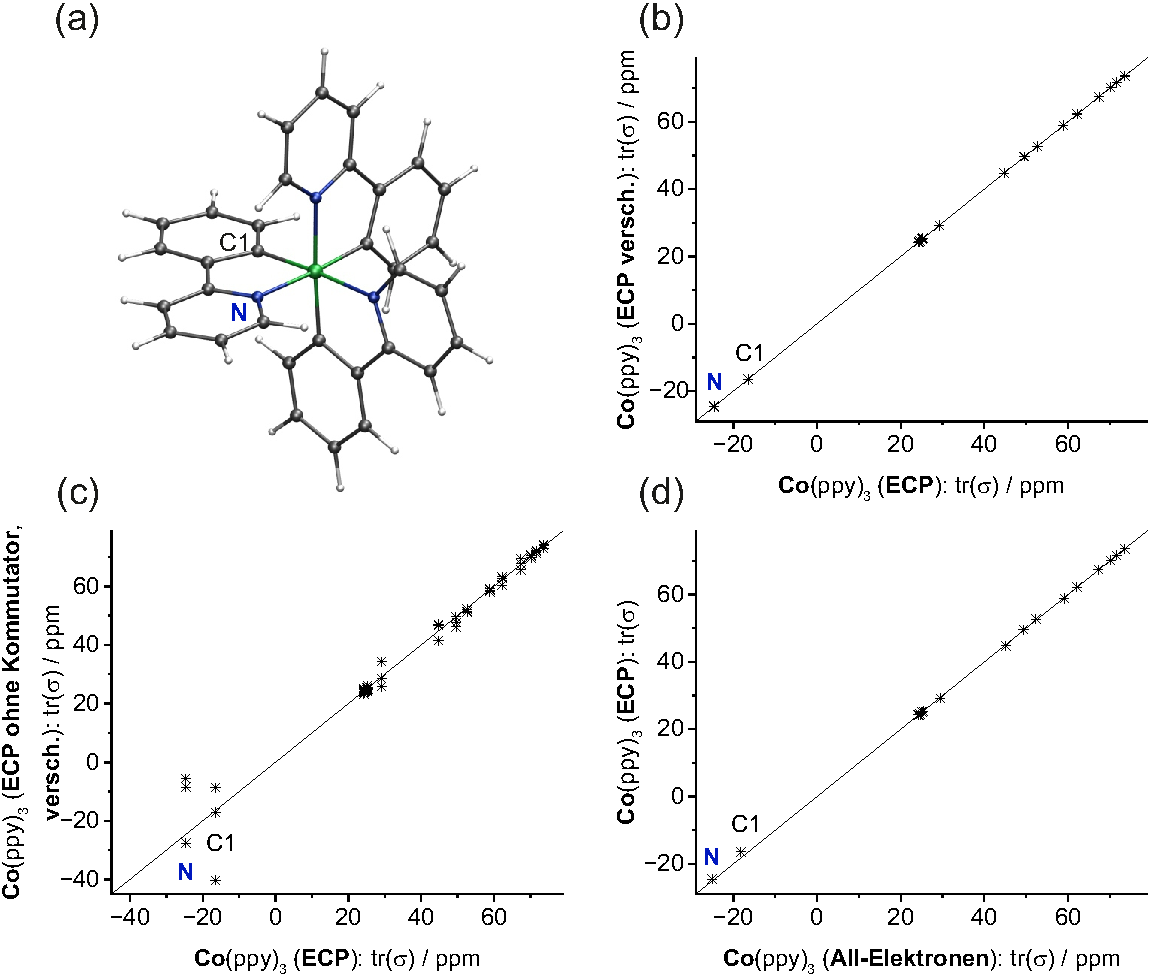
\includegraphics[width=1.0\textwidth]{ecptest}
	\captionsetup{figurewithin = chapter}
	\captionsetup{font=small, labelfont=bf}\caption[ECP-Testrechnungen an Co(ppy)$_3$]{\textbf{Oben links:} Abbildung von Co(ppy)$_3$, ppy=2-Phenylpyridin (Kohlenstoff=grau, Wasserstoff=weiß, Stickstoff=blau und Cobalt=grün). \textbf{Oben rechts:} Chemische Abschirmungskonstanten von Co(ppy)$_3$ berechnet mit \acp{ecp} (y-Achse) gegen die chemischen Abschirmungskonstanten von Co(ppy)$_3$ berechnet mit einer All-Elektronen Basis (x-Achse). \textbf{Unten links:} Chemische Abschirmungen von Co(ppy)$_3$  berechnet mit \acp{ecp}, wobei das Molekül um \unit[10]{a.u.} in Richtung der Raumdiagonalen verschoben wurde (y-Achse) gegen die chemischen Abschirmungskonstanten von Co(ppy)$_3$ berechnet mit \acp{ecp}, wobei das Co-Atom im Koordinatenursprung liegt (x-Achse). \textbf{Unten rechts:} Wie unten links, nur dass die chemischen Abschirmungskonstanten für das verschobene Molekül ohne den Beitrag durch den von van Wüllen hergeleiteten Kommutator berechnet wurden.}
\label{abb:coppy3test}
\end{figure}

Wie bereits in Kapitel \ref{kap:ecps} erwähnt, lassen sich für Atome mit \acp{ecp} keine absoluten chemischen Abschirmungskonstanten berechnen. Jedoch können die Berechneten Abschirmungskonstanten gut mit experimentell gemessenen chemischen Verschiebungen korreliert werden. Dies ist insbesondere dann möglich wenn es sich dabei um ähnliche Systeme handelt. Um dies zu demonstrieren, wurden die Abschirmungskonstanten der Zinnatome in den Verbindungen SnH$_4$, SnMeH$_3$, SnMe$_2$H$_2$, SnMe$_3$H und SnMe$_4$ mit \acp{ecp} berechnet. Die experimentell gemessenen chemischen Verschiebungen dieser Verbindungen wurden Referenz \cite{vivas2002dft} entnommen. In Abbildung \ref{abb:snecpshifts} wurden die mit \ac{ecp} berechneten chemischen Abschirmungskonstanten gegen die experimentell gemessenen Daten aufgetragen. Es ist eindeutig zu erkennen, dass sich die berechneten Werte sehr gut mit den experimentellen korrelieren lassen. Der Absolutwert der chemischen Verschiebung ist jedoch um 1-2 Größenordnungen kleiner, da die wesentlichen Beiträge der Kernnahen Elektronen fehlen. Für diese Berechnungen gelten die selben, oben bereits erwähnten Einstellungen mit der Ausnahme, dass das TPSS Funktional\supercite{tao2003climbing} und die def2-TZVP Basis\supercite{weigend2005balanced} verwendet wurden.
\begin{figure}[ht!]
	\centering
	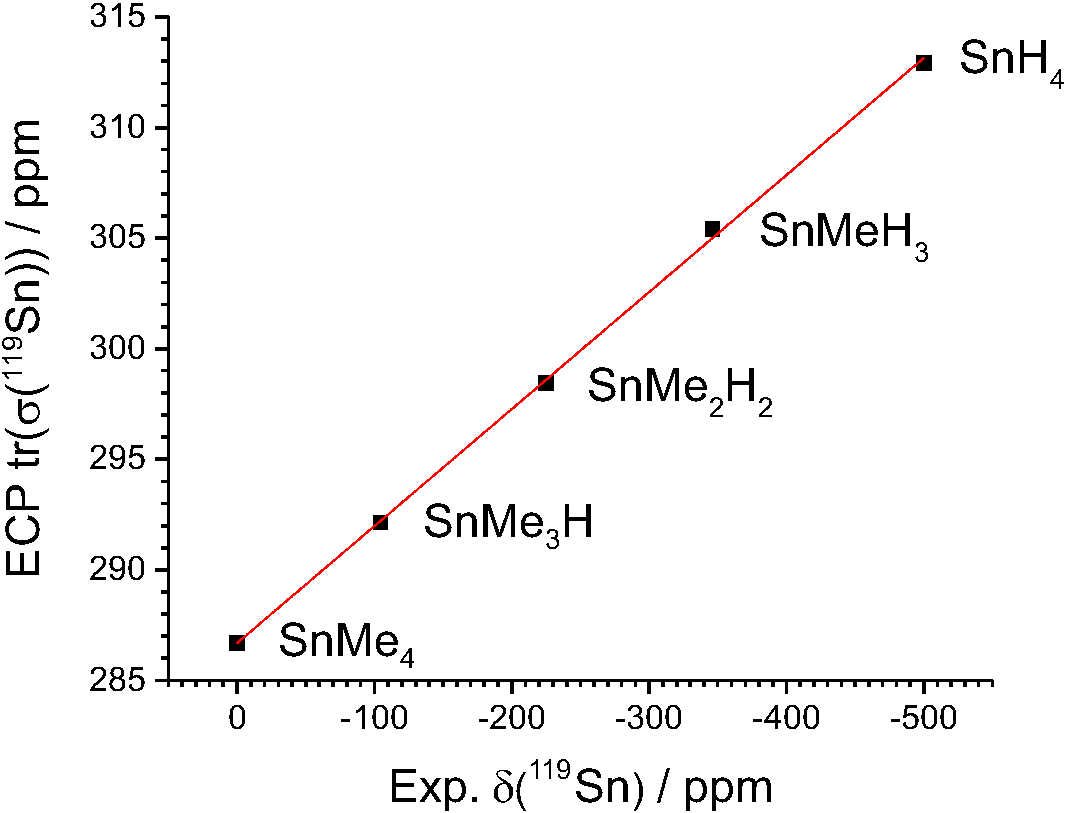
\includegraphics[width=0.6\textwidth]{snecpshifts}
	\captionsetup{figurewithin = chapter}
	\captionsetup{font=small, labelfont=bf}\caption[Vergleich experimenteller $^{119}$Sn Verschiebungen mit berechneten Abschirmungskonstanten]{Vergleich experimenteller $^{119}$Sn Verschiebungen mit berechneten Abschirmungskonstanten mit \acp{ecp}. Die Absolutwerte der Berechneten Abschirmungskonstanten sind um 1-2 Größenordnungen zu gering, jedoch lassen sie sich sehr gut mit den gemessenen Verschiebungen in Korrelation bringen.}
\label{abb:snecpshifts}
\end{figure}
	
\section{Berechnung von Vibrational Circular Dichroism Spektren}
	\subsection{Theorie}
	Die im Experiment gemessenen Intensitäten der \ac{vcd}-Spektroskopie $I_n$ sind proportional zu den in quantenchemischen Rechnungen zugänglichen Rotationsstärken $R_n$. Letztere werden aus dem Skalaprodukt vom elektrischen und vom magnetischen Übergangsdipolmoment, $\vec{\mu}_n^{\,\text{el}}$ und $\vec{\mu}_n^{\,\text{mag}}$,  erhalten. Somit ergibt sich die \ac{vcd}-Intensität
	\begin{equation}\label{eq:rotationsstaerke}
	  I_n\approx R_n = Im(\vec{\mu}_n^{\,\text{el}}\cdot\vec{\mu}_n^{\text{\,mag}})
	\end{equation}
	für einen Übergang aus dem Schwingungsgrundzustand in den angeregten Schwingungszustand $n$.\supercite{stephens1985theory,stephens1985vibrational} Im Rahmen der harmonishen Näherung sind das elektrische und das magnetische Übergangsdipolmoment gegeben durch\supercite{cheeseman1996ab,nicu2008vibrational}
	
	\begin{equation}\label{eq:eludm}
	  (\mu_n^{\text{el}})_\beta=\sqrt{\frac{\hbar}{\omega_n}}\sum_{K\alpha}P_{\alpha\beta}^K S_{K\alpha,n}
	\end{equation}
	\begin{equation}\label{eq:magudm}
	  (\mu_n^{\text{mag}})_\beta=-\sqrt{2\hbar^3\omega_n}\sum_{K\alpha}M_{\alpha\beta}^KS_{K\alpha,n}.
	\end{equation}
	Hierbei ist $I$ die Zählvariable für die Atomkerne, $\alpha$ und $\beta$ beschreiben kartesische Koordinaten, $\omega_n$ ist die Schwingungsfrequenz der $n$-ten Schwingung und $S_{I\alpha,n}$ ist die Transformationsmatrix von kartesichen zu Normalkoordinaten. Sowohl der sogenannte \ac{apt} (Gleichung (\ref{eq:apt})) als auch der sogenannte \ac{aat} (Gleichung (\ref{eq:aat})) lassen sich in einen elektronischen und einen Kernbeitrag aufteilen
	\begin{equation}\label{eq:apt}
	  P^K_{\alpha\beta}=E^K_{\alpha\beta}+N^K_{\alpha\beta}
	\end{equation}
	\begin{equation}\label{eq:aat}
   	  M^K_{\alpha\beta}=I^K_{\alpha\beta}+J^K_{\alpha\beta}.
	\end{equation}
	Die Berechnung der Kernbeiträge 
	\begin{equation}
	  N^K_{\alpha\beta}=eZ_K\delta_{\alpha\beta}
	\end{equation}
	\begin{equation}\label{eq:aatkern}
	  J^K_{\alpha\beta}=\iu\frac{eZ_K}{4\hbar c}\sum_K^{N_K}\varepsilon_{\alpha\beta\gamma}R^0_{K\gamma}
	\end{equation}
	ist trivial. $e$ ist die Elementarladung, $Z_K$ ist die Ladung des Kerns $K$ und $\delta_{\alpha\beta}$ ist das Kroneckerdelta. $c$ ist die Lichtgeschwindigkeit und $\varepsilon_{\alpha\beta\gamma}$ ist der Levi-Civita-Permutationstensor. Die Position des Kerns $K$ ist durch $R^0_{K\gamma}$ gegeben, wobei $\gamma$ für eine der drei kartesischen Raumkoordinaten steht und die hochgestellte $0$ symbolisiert die Auswertung in der Gleichgewichtsgeometrie.   
	
    Zur Berechnung der elektronischen Beiträge 
    \begin{equation}
      E^K_{\alpha\beta}=\left(\sum_{i=1}^{N_{\text{occ}}}\frac{\partial \langle\phi_i\vert r_\beta\vert\phi_i\rangle}{\partial R_{K\alpha}}\right)_{\vec{R}^0}
    \end{equation}
    \begin{equation}\label{eq:vcdaatel}
      I^K_{\alpha\beta}=\sum_{i=1}^{N_{\text{occ}}}=\left\langle\left.\left(\frac{\partial \phi_i}{\partial R_{K\alpha}}\right)_{\vec{R}^0}\right|\left(\frac{\partial \phi_i}{\partial B_\beta}\right)_{\vec{B}=0}\right\rangle
    \end{equation}
    
    ist ein deutlich größerer Aufwand erforderlich. Die $\phi_i$ sind die besetzten \acp{mo}. Wie bereits in Kapitel \ref{theo:nmr} beschrieben, lasst sich die \ac{mo}-Ableitung nach einer Komponente des externen magnetischen Feldes im Rahmen des \ac{cphf}-Formalismus als 
    \begin{equation}\label{eq:vcdcphf}
    \left(\frac{\partial \phi_i}{\partial B_\beta}\right)_{\vec{B}=0}=\phi_i^{B_\beta}=\sum_{\mu=1}^{N_{\text{BF}}}\left[c_{\mu i}\chi_\mu^{B_\beta}+\sum_{p=1}^{N_{\text{MO}}}c_{\mu p}U_{ip}^{B_\beta}\chi_\mu\right]
	\end{equation}
	ausdrücken. Die Koeffizientenmatrix $U_{ip}^{B_\beta}$ beschreibt die Änderung der Molekülorbitale durch die Störung des äußeren Magnetischen Feldes $\vec{B}$. Sie wird durch Lösen der entsprechenden \ac{cphf}-Gleichungen erhalten, ganz analog zur Vorgehensweise bei der Berechnung von \ac{nmr}-Abschirmkonstanten. Durch die Kombination der Gleichungen (\ref{eq:vcdaatel}) und  (\ref{eq:vcdcphf}) wird der zu implementierende Ausdruck für den elektronischen Anteil des \ac{aat} erhalten
	\begin{equation}\label{eq:vcdaatelfinal}
	\begin{aligned}
	I^K_{\alpha\beta}=&\sum_{i=1}^{N_{\text{occ}}}\sum_{\mu,\nu=1}^{N_{\text{BF}}}\left[c_{\mu i}c_{\nu i}\left\langle\chi_\mu^{R_{K\alpha}}\vert\chi_\nu^{B_\beta}\right\rangle+\sum_{p=1}^{N_{\text{MO}}}c_{\mu i}c_{\nu p}U_{ip}^{B_\beta}\left\langle\chi_\mu^{R_{K\alpha}}\vert\chi_\nu\right\rangle\right.\\
	&\left.+\sum_{p=1}^{N_{\text{MO}}}c_{\mu i}c_{\nu p}U_{ip}^{R_{K_\alpha}}\left\langle\chi_\mu\vert\chi_\nu^{B_{\beta}}\right\rangle+\sum_{p,q=1}^{N_{\text{MO}}}c_{\mu p}c_{\nu q}U_{ip}^{R_{K_\alpha}}U_{iq}^{B_\beta}\left\langle\chi_\mu\vert\chi_\nu\right\rangle\right].
	\end{aligned}
	\end{equation}
	Durch die Koeffizientenmatrix $U_{ip}^{R_{K_\alpha}}$ wird die Response der Wellenfunktion auf die Verrückung des Kerns $K$ beschrieben. Analog zu $U_{ip}^{B_\beta}$ werden auch sie durch Lösen der entsprechenden \ac{cphf}-Gleichungen erhalten. Gebraucht werden sie ebenfalls zur Berechnung von Kraftkonstanten, wie sie im \textsc{Turbomole} Modul \texttt{aoforce}\supercite{deglmann2002efficient} berechnet werden.
	\subsection{Implementierung}
Die Implementierung zur Berechnung von \ac{vcd}-Spektren lässt sich am Einfachsten durch folgende zwei Schritte realisieren. Im ersten Schritt wird die Koeffizientenmatrix $U_{ip}^{B_\beta}$ im Modul \texttt{mpshift} berechnet und auf der Festplatte gespeichert. Diese wird vom Modul \texttt{aoforce} eingelesen, welches ebenfalls alle notwendigen Integrale, die $U_{ip}^{R_{K_\alpha}}$, den \ac{aat}(Gleichung \ref{eq:aat}) und den \ac{apt} (Gleichung \ref{eq:apt}) berechnet. Letzterer wird bereits für die Berechnung von \ac{ir}-Intensitäten benötigt und steht daher im Modul \texttt{aoforce} bereits zu Verfügung. Aus dem \ac{aat} und dem \ac{apt} lassen sich schließlich die eigentlichen \ac{vcd}-Intensitäten berechnen. Der Hauptaufwand liegt daher in der Implementierung des \ac{aat} nach Gleichung (\ref{eq:vcdaatelfinal}). Das Integral im vierten Term dieser Gleichung ist ein Standard Überlappungsintegral und das Integral im zweiten Term ist das nach den Kernkoordinaten abgeleitete Überlappungsintegral. Auch disese Integrale stehen im Modul \texttt{aoforce} bereits zur Verfügung.	Die in Gleichung (\ref{eq:vcdaatelfinal}) auftretenden Integrale, welche die Ableitung nach dem externen magnetischen Feld enthalten, lassen sich wie folgt umschreiben

	\begin{equation}\label{eq:ddipx}
	\begin{aligned}
	\left\langle\chi_\mu^{R_{K_\alpha}}\vert\chi_\nu^{B_x}\right\rangle&=\left.\left\langle\chi_\mu^{R_{K_\alpha}}\left|\frac{\partial}{\partial B_x}\right.\chi_\nu\right\rangle\right|_{\vec{B}=0}=\left\langle\chi_\mu^{R_{K_\alpha},\vec{B}=0}\left|\frac{-\iu}{2c}\left(R_{\nu y}z-R_{\nu z}y\right)\right|\chi_\nu^{\vec{B}=0}\right\rangle\\
	  &=\frac{\iu}{2c}\left(R_{\nu z}\left\langle\chi_\mu^{R_{K_\alpha},\vec{B}=0}\left|y\right|\chi_\nu^{\vec{B}=0}\right\rangle-R_{\nu y}\left\langle\chi_\mu^{R_{K_\alpha},\vec{B}=0}\left|z\right|\chi_\nu^{\vec{B}=0}\right\rangle\right).
	  \end{aligned}
	\end{equation}
	
	Analog ergeben sich die Ableitungen nach der $y$-
	\begin{equation} \label{eq:ddipy}
	\left\langle\chi_\mu^{R_{K_\alpha}}\vert\chi_\nu^{B_y}\right\rangle=\frac{\iu}{2c}\left(R_{\nu x}\left\langle\chi_\mu^{R_{K_\alpha},\vec{B}=0}\left|z\right|\chi_\nu^{\vec{B}=0}\right\rangle-R_{\nu z}\left\langle\chi_\mu^{R_{K_\alpha},\vec{B}=0}\left|x\right|\chi_\nu^{\vec{B}=0}\right\rangle\right)
	\end{equation}
	
	und $z$-Komponente	
	\begin{equation} \label{eq:ddipz}
	\left\langle\chi_\mu^{R_{K_\alpha}}\vert\chi_\nu^{B_z}\right\rangle=\frac{\iu}{2c}\left(R_{\nu y}\left\langle\chi_\mu^{R_{K_\alpha},\vec{B}=0}\left|x\right|\chi_\nu^{\vec{B}=0}\right\rangle-R_{\nu x}\left\langle\chi_\mu^{R_{K_\alpha},\vec{B}=0}\left|y\right|\chi_\nu^{\vec{B}=0}\right\rangle\right).
	\end{equation}
	Das zweite auftretende Integral (Term drei in Gleichung (\ref{eq:vcdaatelfinal})) ist für die einzelnen Komponenten gegeben durch	
	\begin{equation} \label{eq:dipx}
	\begin{aligned}
	  \left\langle\chi_\mu\vert\chi_\nu^{B_x}\right\rangle&=\left.\left\langle\chi_\mu\left|\frac{\partial}{\partial B_x}\right.\chi_\nu\right\rangle\right|_{\vec{B}=0}=\left\langle\chi_\mu^{\vec{B}=0}\left|\frac{-\iu}{2c}\left(R_{\nu y}z-R_{\nu z}y\right)\right|\chi_\nu^{\vec{B}=0}\right\rangle\\
	  &=\frac{\iu}{2c}\left(R_{\nu z}\left\langle\chi_\mu^{\vec{B}=0}\left|y\right|\chi_\nu^{\vec{B}=0}\right\rangle-R_{\nu y}\left\langle\chi_\mu^{\vec{B}=0}\left|z\right|\chi_\nu^{\vec{B}=0}\right\rangle\right),
	\end{aligned}
	\end{equation}
 
		\begin{equation} \label{eq:dipy}
	  \left\langle\chi_\mu\vert\chi_\nu^{B_y}\right\rangle=\frac{\iu}{2c}\left(R_{\nu x}\left\langle\chi_\mu^{\vec{B}=0}\left|z\right|\chi_\nu^{\vec{B}=0}\right\rangle-R_{\nu z}\left\langle\chi_\mu^{\vec{B}=0}\left|x\right|\chi_\nu^{\vec{B}=0}\right\rangle\right),
	\end{equation}
	
		\begin{equation} \label{eq:dipz}
	  \left\langle\chi_\mu\vert\chi_\nu^{B_z}\right\rangle=\frac{\iu}{2c}\left(R_{\nu y}\left\langle\chi_\mu^{\vec{B}=0}\left|x\right|\chi_\nu^{\vec{B}=0}\right\rangle-R_{\nu x}\left\langle\chi_\mu^{\vec{B}=0}\left|y\right|\chi_\nu^{\vec{B}=0}\right\rangle\right).
	\end{equation}

	

	Die Integrale in den Gleichungen (\ref{eq:ddipx})-(\ref{eq:dipz}) lassen sich damit entsprechend durch eine Linearkombination von gewöhnlichen Dipolintegralen $\langle\chi_\mu\vert\vec{r}\vert\chi_\nu\rangle$ und nach den Kernkoodinaten abgeleiteten Dipolintegralen $\langle\chi_\mu^{R_{K_\alpha}}\vert\vec{r}\vert\chi_\nu\rangle$ ausdrücken. Diese werden bereits im Modul \texttt{aoforce} berechnet und müssen daher nur auf geeignete Weise kombiniert werden, um die nach den Komponenten des Magnetfeldes abgeleiteten Integrale zu erhalten. Mit den \ac{mo}-Koeffizienten lassen sich die Integrale in den Termen drei und vier aus der \ac{cao}-Basis in die \ac{mo}-Basis transformieren und zusammenfassen\supercite{nicu2008vibrational}
	
	\begin{equation}\label{eq:term3+4}
	\begin{aligned}
	&\sum_{\mu,\nu=1}^{N_{\text{BF}}}\left[\sum_{p=1}^{N_{\text{MO}}}c_{\mu i}c_{\nu p}U_{ip}^{R_{K_\alpha}}\left\langle\chi_\mu\vert\chi_\nu^{B_{\beta}}\right\rangle+\sum_{p,q=1}^{N_{\text{MO}}}c_{\mu p}c_{\nu q}U_{ip}^{R_{K_\alpha}}U_{iq}^{B_\beta}\left\langle\chi_\mu\vert\chi_\nu\right\rangle\right]\\
	&=\sum_{p=1}^{N_{\text{MO}}}U_{ip}^{R_{K_\alpha}}S_{ip}^{B_\beta}+\sum_{p,q=1}^{N_{\text{MO}}}U_{ip}^{R_{K_\alpha}}U_{iq}^{B_\beta}\delta_{pq}\\
	&=\sum_{p=1}^{N_{\text{MO}}}U_{ip}^{R_{K_\alpha}}S_{ip}^{B_\beta}+\sum_{p=1}^{N_{\text{MO}}}U_{ip}^{R_{K_\alpha}}U_{ip}^{B_\beta}\\
	&=\sum_{p=1}^{N_{\text{MO}}}U_{ip}^{R_{K_\alpha}}\left(S_{ip}^{B_\beta}+U_{ip}^{B_\beta}\right).
	\end{aligned}
	\end{equation}
	Die Abbildung \ref{abb:programmstrukur_vcd} zeigt wieder eine schematische Darstellung der wichtigsten Routinen für die Berechnung von \ac{vcd}-Spektren. Ihre genaue Funktion wird im folgenden erläutert. 
\begin{itemize}
	\item[\texttt{wrumunu}:] Transformation der $U_{ip}^{B_\beta}$ in die \ac{cao}-Basis. Anschließend werden die $U_{\mu\nu}^{B_/beta}$ in der Datei \texttt{umunu} auf der Festplatte gespeichert.
	\item[\texttt{scf2nd}:] Übergeordnete Routine zur Lösung der \ac{cphf}-Gleichungen für die $U_{ip}^{R_{K_\alpha}}$.
	\item[\texttt{dipai}:] Berechnung der Integrale in den Gleichungen (\ref{eq:dipx}) bis (\ref{eq:dipz}) aus den Dipolintegralen.
	\item[\texttt{dinumu}:] Übergeordnete Routine zur Berechnung der Dipolintegrale und der nach den Kernkoordinaten abgeleiteten Dipolintegrale.
	\item[\texttt{dipdrv}:] Berechnung der Integrale in den Gleichungen (\ref{eq:ddipx}) bis (\ref{eq:ddipz}) aus den nach den Kernkoordinaten abgeleiteten Dipolintegralen für den ersten Term auf der rechten Seite von Gleichung (\ref{eq:vcdaatelfinal}).
	\item[\texttt{gocart}:] Berechnung der ungestörten Überlappungsmatrix.
	\item[\texttt{dipsijxi}:] Übergeordnete Routine zur Berechnung des Produkts $U_{ij}^{R_{K_\alpha}}\left(S_{ij}^{B_\beta}+U_{ij}^{B_\beta}\right)$ aus Gleichung (\ref{eq:term3+4}) bzw. die Terme drei und vier aus der Gleichung (\ref{eq:vcdaatelfinal}) für den besetzt-besetzt-Block. $S_{ij}^{B_\beta}+U_{ij}^{B_\beta}$ wird in \texttt{rdumunu} berechnet, das Produkt in \texttt{mijxidip}.
	\item[\texttt{rdumunu}:] Einlesen der $U_{\mu\nu}^{B_\beta}$ aus der Datei \texttt{umunu}. Anschließend erfolgt die Rücktransformation in die \ac{mo}-Basis sowie die Zerlegung in den besetzt-besetzt- bzw. besetzt-virtuell-Block. Des Weiteren werden an dieser Stelle auch die nach den Komponenten des Magnetfeldes abgeleiteten Überlappungsmatrizen aus den Gleichungen (\ref{eq:dipx}) bis (\ref{eq:dipz}) in die \ac{mo}-Basis transformiert. Schließlich erfolgt die Berechnung von $S_{ij}^{B_\beta}+U_{ij}^{B_\beta}$ und $S_{ia}^{B_\beta}+U_{ia}^{B_\beta}$.
	\item[\texttt{mijxidip}:] Eigentliche Berechnung des Produkts $U_{ij}^{R_{K_\alpha}}\left(S_{ij}^{B_\beta}+U_{ij}^{B_\beta}\right)$ für den besetzt-besetzt-Block.
	\item[\texttt{dipuaixi}:] Übergeordnete Routine zur Berechnung des Produkts $U_{ia}^{R_{K_\alpha}}\left(S_{ia}^{B_\beta}+U_{ia}^{B_\beta}\right)$ aus Gleichung (\ref{eq:term3+4}) bzw. die Terme drei und vier aus der Gleichung (\ref{eq:vcdaatelfinal}) für den besetzt-virtuell-Block. $S_{ia}^{B_\beta}+U_{ia}^{B_\beta}$ wird in \texttt{rdumunu} berechnet, das Produkt in \texttt{maixidip}.
	\item[\texttt{maixidip}:] Eigentliche Berechnung des Produkts $U_{ia}^{R_{K_\alpha}}\left(S_{ia}^{B_\beta}+U_{ia}^{B_\beta}\right)$ für den besetzt-virtuell-Block.
	\item[\texttt{vibro}:] Übergeordnete Routine zur Berechnung des \ac{apt}, der \ac{vcd}-Rotationsstärken und Ausgabe der Ergebnisse.
	\item[\texttt{prtnpr}:] Übergeordnete Routine zur Steuerung der Ergebnisausgabe. 
	\item[\texttt{wrtfrq}:] Ausgabe der \ac{vcd}-Rotationsstärken in der Datei \texttt{vibspectrum} in \unit[1$\times 10^{-44}$]{$esu^2cm^2$}.
	\item[\texttt{vibfrq}:] Übergeordnete Routine zur Berechnung des \ac{apt}, der \ac{vcd}-Rotationsstärken und Ausgabe der Ergebnisse.
	\item[\texttt{rotvib}:] Berechnung des \ac{apt} nach Gleichung (\ref{eq:apt}) aus den nach den Kernkoordinaten abgeleiteten Dipolintegralen mit anschließender Transformation von kartesischen Koordinaten auf Normalkoordinaten nach Gleichung (\ref{eq:eludm})
	\item[\texttt{mkvcd}:] Berechnung der eigentlichen \ac{vcd}-Rotationsstärken aus den bisherigen Zwischengrößen. Zuerst werden die nach den Komponenten der Kernkoordinaten abgeleitete Überlappungsmatrix $S_{\mu\nu}^{R_{K_\alpha}}=\left\langle\chi_\mu^{R_{K_\alpha}}\vert\chi_\nu\right\rangle$ und $U_{\mu\nu}^{B_\beta}$ in der \ac{cao}-Basis aus den Dateien \texttt{dS} und \texttt{umunu} eingelesen. Diese werden für den zweiten Term des \ac{aat} auf der rechten Seite von Gleichung (\ref{eq:vcdaatelfinal}) benötigt. Anschließend wird das Produkt $U_{\mu\nu}^{B_\beta}S_{\mu\nu}^{R_{K_\alpha}}$ gebildet. Als letzter für den \ac{aat} verbleibender Term, wird der triviale Kernbeitrag nach Gleichung (\ref{eq:aatkern}) berechnet. Aus allen bisher berechneten Zwischengrößen (Term eins: \texttt{dipdrv}, Term zwei: \texttt{mkvcd}, Term drei und vier: \texttt{dipsijxi} und \texttt{dipsijxi}, Kernbeitrag: \texttt{mkvcd}) kann schließlich der gesamte \ac{aat} gebildet werden. Nach der Transformation des \ac{aat} von kartesischen Koordinaten auf nach Normalkoordinaten (Gleichung (\ref{eq:magudm})) werden die Rotationsstärken durch Skalarmultiplikation des \ac{aat} mit dem \ac{apt} nach Gleichung (\ref{eq:rotationsstaerke}) erhalten.  
	\item[\texttt{prtram}:] Ausgabe der \ac{vcd}-Rotationsstärken in der Standard Programmausgabe in \unit[1$\times 10^{-44}$]{$esu^2cm^2$}.
\end{itemize}
	
	\begin{figure}[ht!]
	\centering
	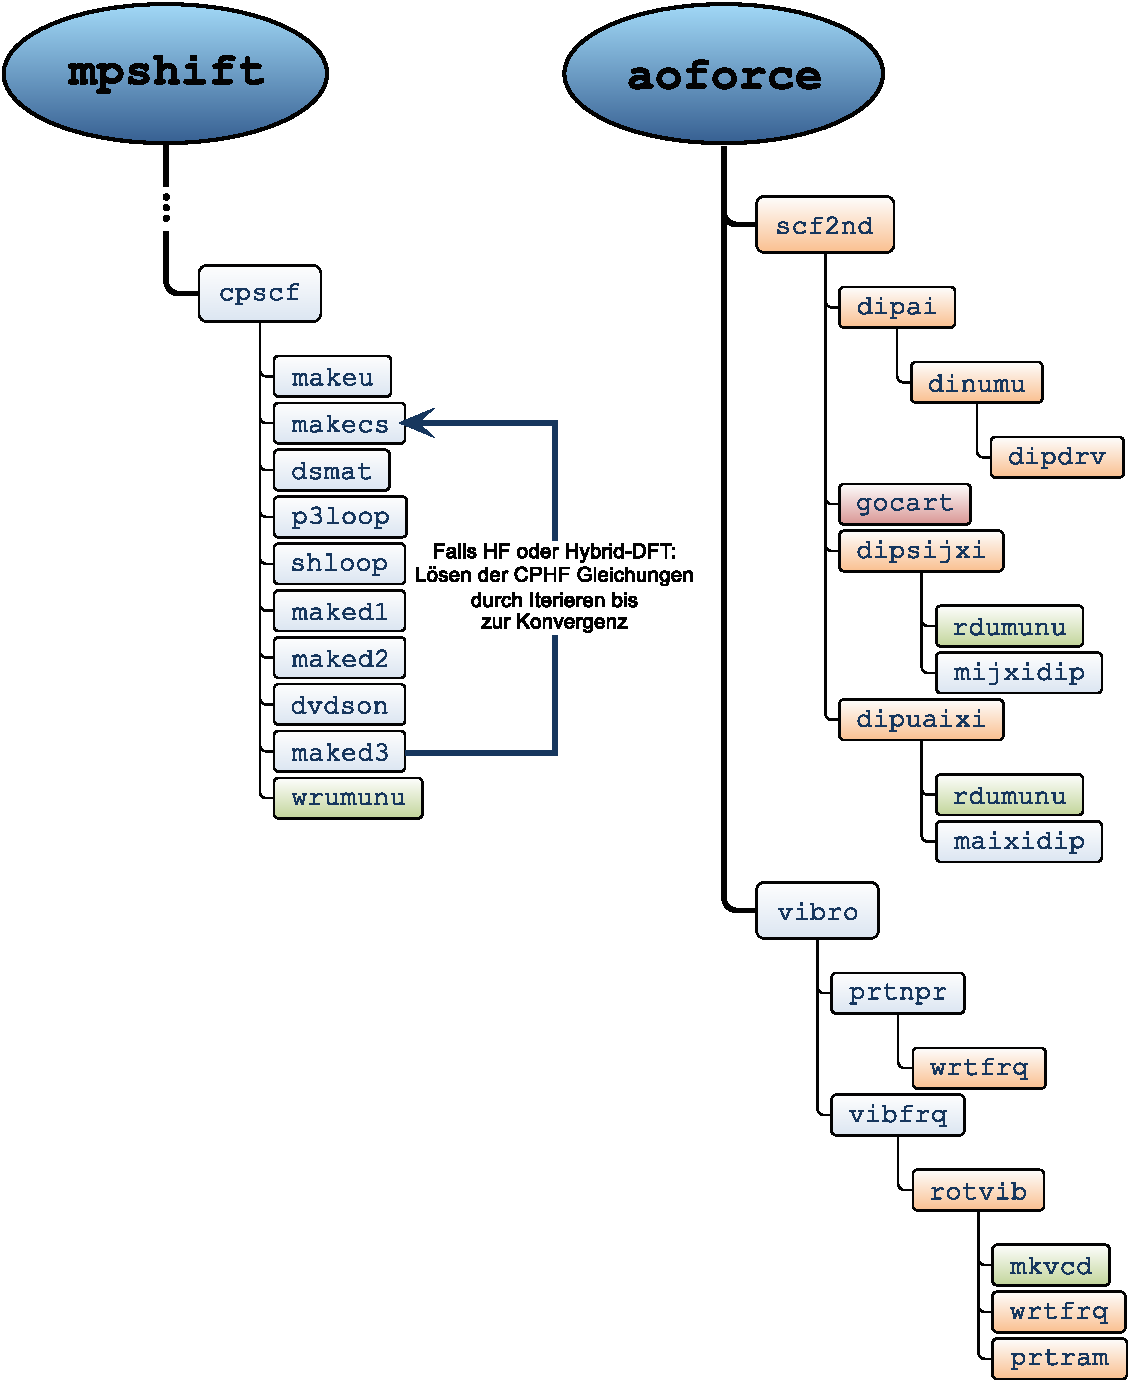
\includegraphics[width=0.95\textwidth]{vcd}
	\captionsetup{figurewithin = chapter}
	\captionsetup{font=small, labelfont=bf}\caption[Wichtigste Routinen für die Berechnung von VCD-Intensitäten]{Schematische Darstellung der wichtigsten Routinen für die Berechnung von \ac{vcd}-Intensitäten in den Modulen \texttt{mpshift} und \texttt{aoforce}. Alte Routinen sind in blau, neue Routinen in grün, modifizierte Routinen in orange und unverändert übertragene Routinen in rot dargestellt.}
\label{abb:programmstrukur_vcd}
\end{figure}	   
	
	
	\subsubsection{Symmetrieausnutzung}
	Nur wenige chirale Moleküle besitzen eine Symmetrie. Sie gehören alle zu den Punktgruppen $C_{\textrm{n}}$, $D_{\textrm{n}}$, $T$, $O$ oder $I$ und besitzen damit nur Drehachsen als Symmetrieelemente. Die bereits bestehende Implementierung der Symmetrieausnutzung\supercite{haser1991molecular} für die Module \texttt{mpshift} und \texttt{aoforce} kann auch für die Berechnung von \ac{vcd} Spektren verwendet werden. Dabei ist jedoch zu beachten, dass die Symmetrieausnutzugn im Modul \texttt{mpshift} keine Punktgruppen mit reduziblen $e$-Darstellungen unterstützt, was die Punktgruppen $C_{\textrm{n>2}}$ und $T$ unter den chiralen Punktgruppen betrifft. In diesen Fällen werden die \ac{mo}-Koeffizienten nach $C_1$ transformiert und \texttt{mpshift} wird ohne Symmetrieausnutzung verwendet. Die $U_{pi}^{B_\beta}$ Koeffizienten werden in die \ac{cao}-Basis transformiert, bevor sie für die Weiterverarbeitung im Modul \texttt{aoforce} auf der Festplatte gespeichert werden. Letzteres unterstützt die volle Symmetrieausnuztung, was wichtig ist, in Anbetracht der Tatsache, dass dies den zeitbestimmenden Schritt darstellt. In \texttt{aoforce} erfolgt die Berechnung der $U_{pi}^{R_{K_\alpha}}$, die $U_{pi}^{B_\beta}$ werden von der Festplatte eingelesen und für die volle Symmetrieausnutzung in die \ac{sao}-Basis transformiert. Abschließend erfolgt die Berechnung der \ac{vcd}-Intensitäten. 
	\subsection{GALLIER: Visualisierung von VCD Spektren}
	Zur Visualisierung der berechneten \ac{vcd}-Intensitäten und um einen schnellen, ersten Eindruck vom \ac{vcd}-Spektrum zu verschaffen, wurde das Pythonskript \ac{gallier} erstellt. Die berechneten \ac{vcd}-Intensitäten und die korrespondierenden Frequenzen werden von dem Skript eingelesen und können im Anschluss daran mit Gauß- oder Lorentzförmigen Kurven verbreitert werden, wodurch ein simuliertes Spektrum erhalten wird. Der Benutzer hat dabei die Wahl ob nur die Intensitäten, nur das simulierte Spektrum oder beides visualisiert werden soll. Standardmäßig wird dafür die von \texttt{aoforce} ausgegebene Datei \texttt{vibspectrum} eingelesen, wodurch auch simultan (oder ausschließlich) das Infrarotspektrum des untersuchten Moleküls visualisiert werden kann. Außerdem besteht zusätzlich die Möglichkeit eine beliebige $x,y$-Datei einzulesen um ein beliebiges Spektrum zu simulieren. \ac{gallier} erzeugt dafür ein Eingabeskript für das Visualisierungsprogramm gnuplot\supercite{gnuplot}, sowie eine Datei mit den Rohdaten für jedes beliebige Visualisierungsprogramm. Die Halbwertsbreite sowie der zu zeichnende Bereich des Spektrums können direkt in \ac{gallier} ausgewählt werden.
	\subsection{Testrechnungen}
	\ac{cpa}
\begin{figure}[ht!]
	\centering
	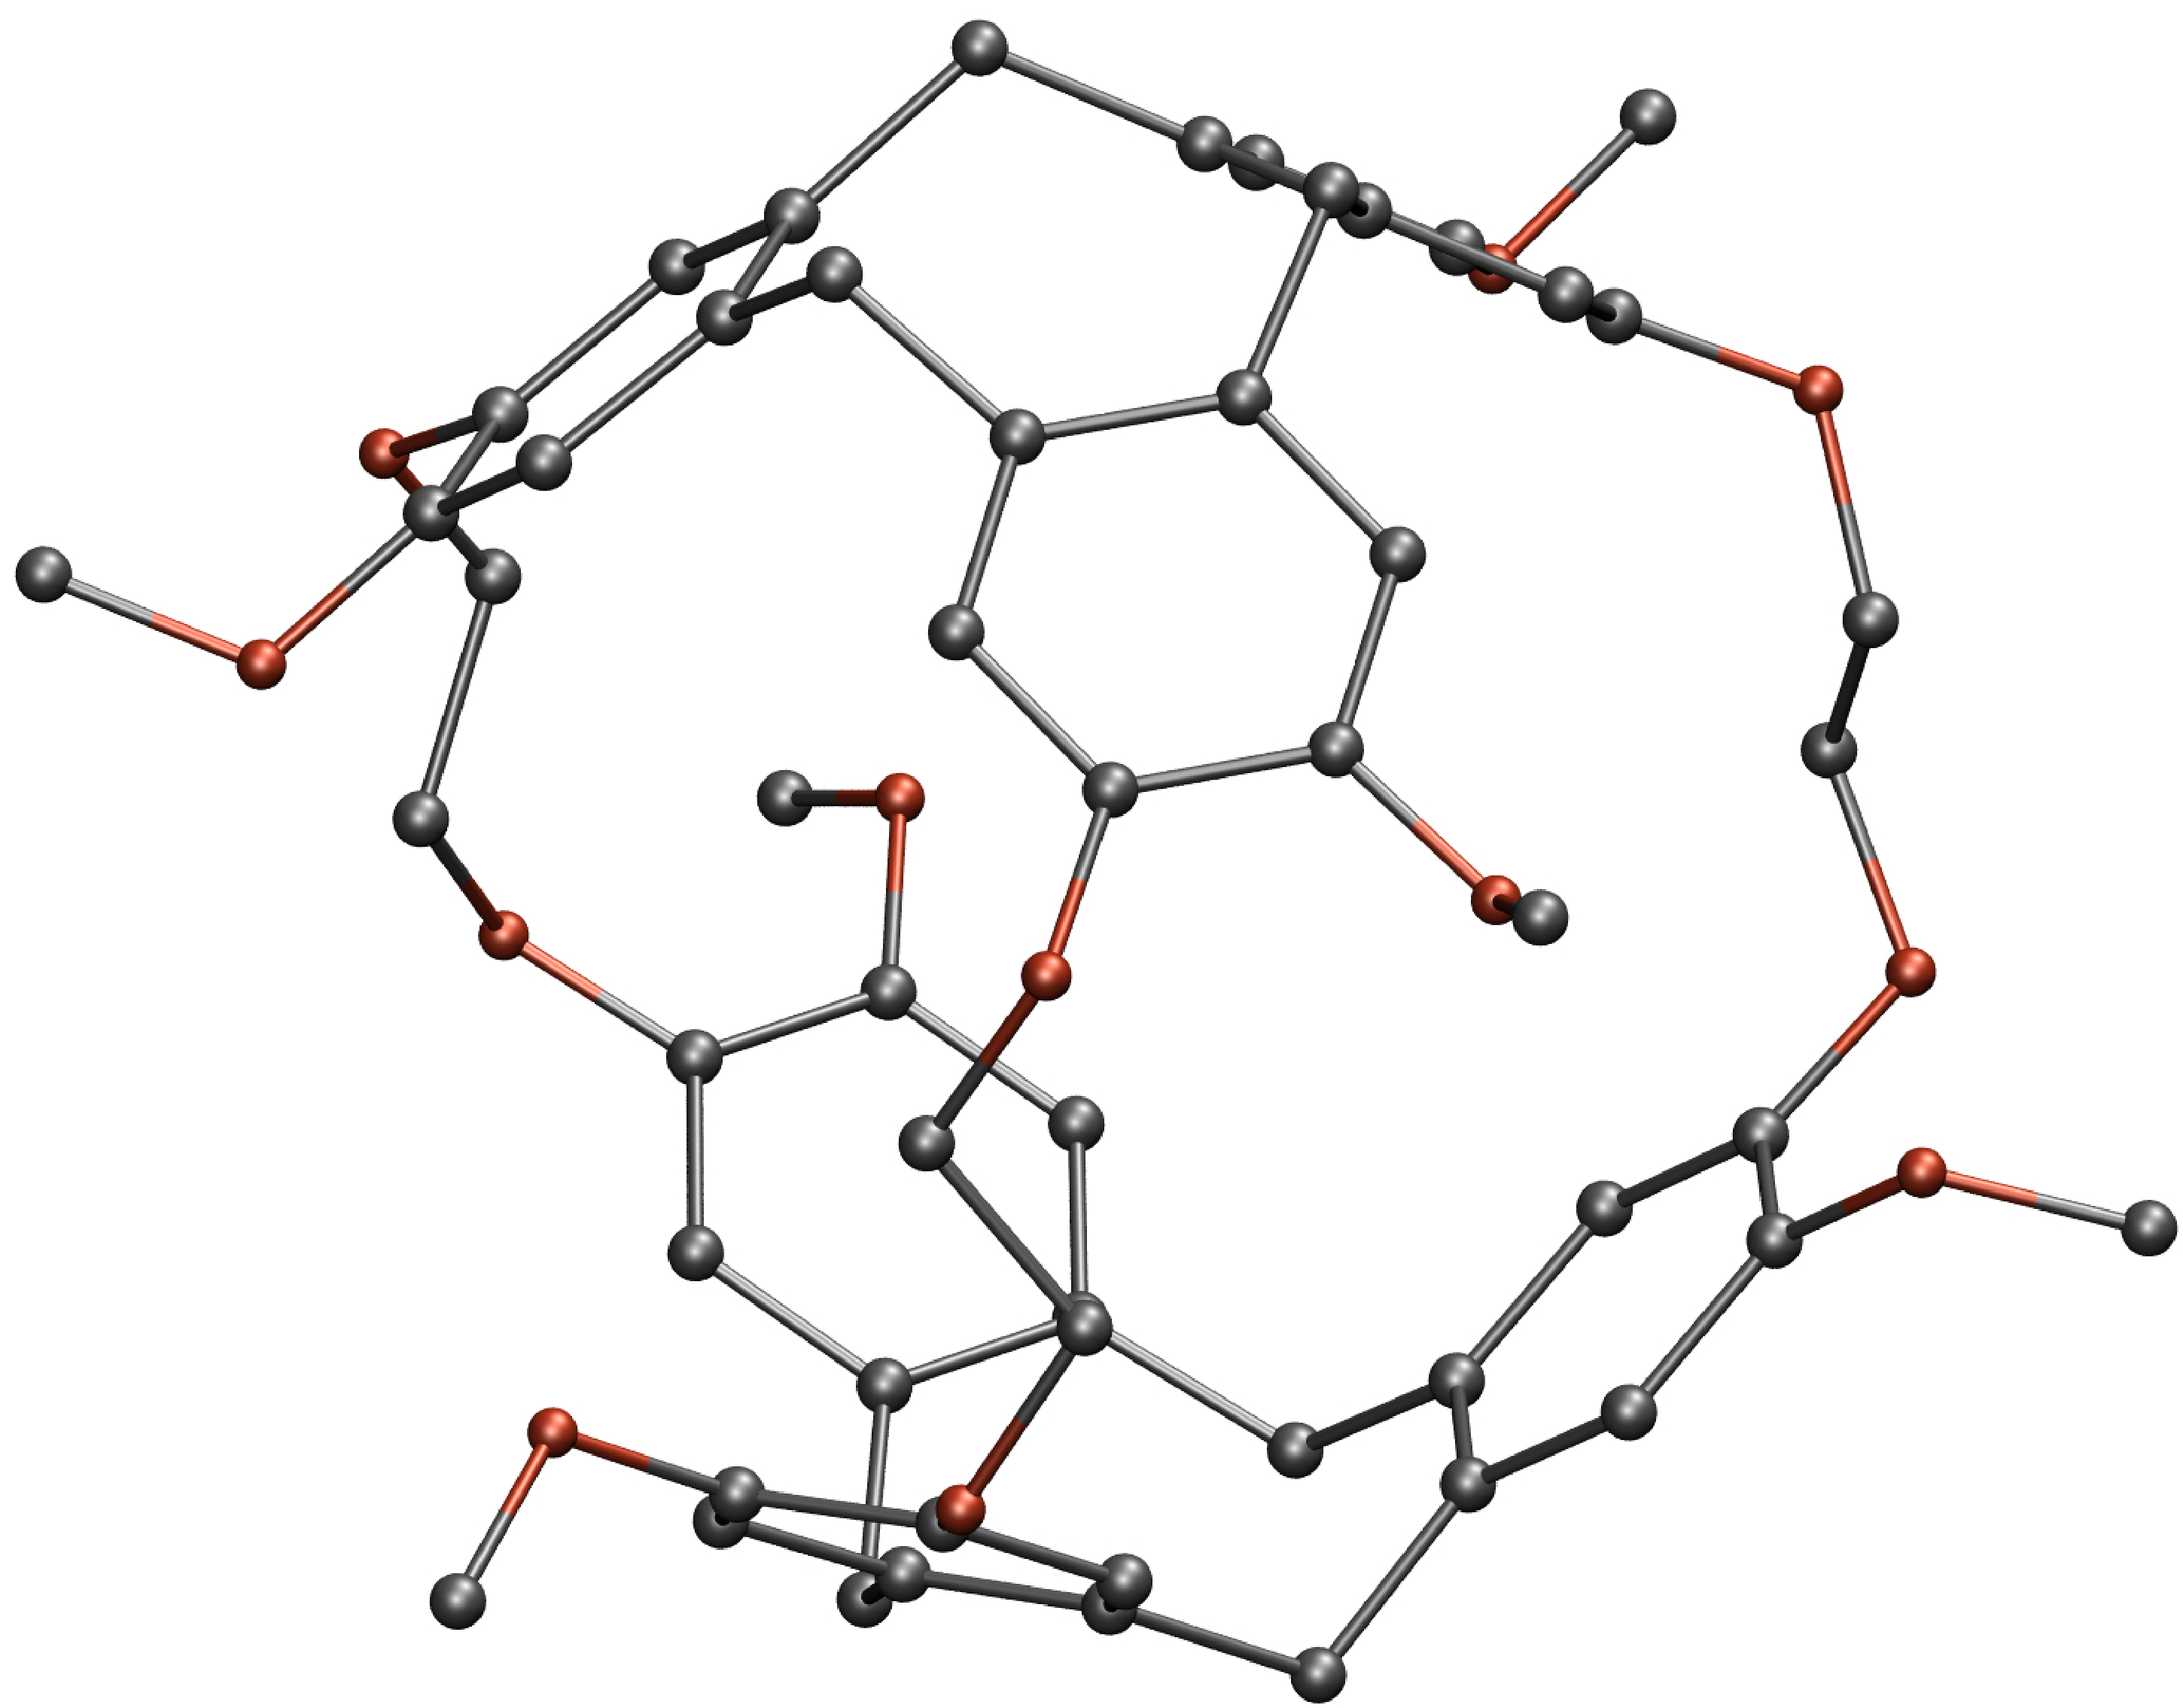
\includegraphics[width=0.6\textwidth]{cpa}
	\captionsetup{figurewithin = chapter}
	\captionsetup{font=small, labelfont=bf}\caption[Abbildung von \ac{cpa}]{Abbildung von \ac{cpa} (Kohlenstoff=grau, Sauerstoff=rot). Die Wasserstoffatome wurden zur besseren Veranschaulichung bei der Abbildung weg gelassen.}
\label{abb:cpa}
\end{figure}

\begin{figure}[ht!]
	\centering
	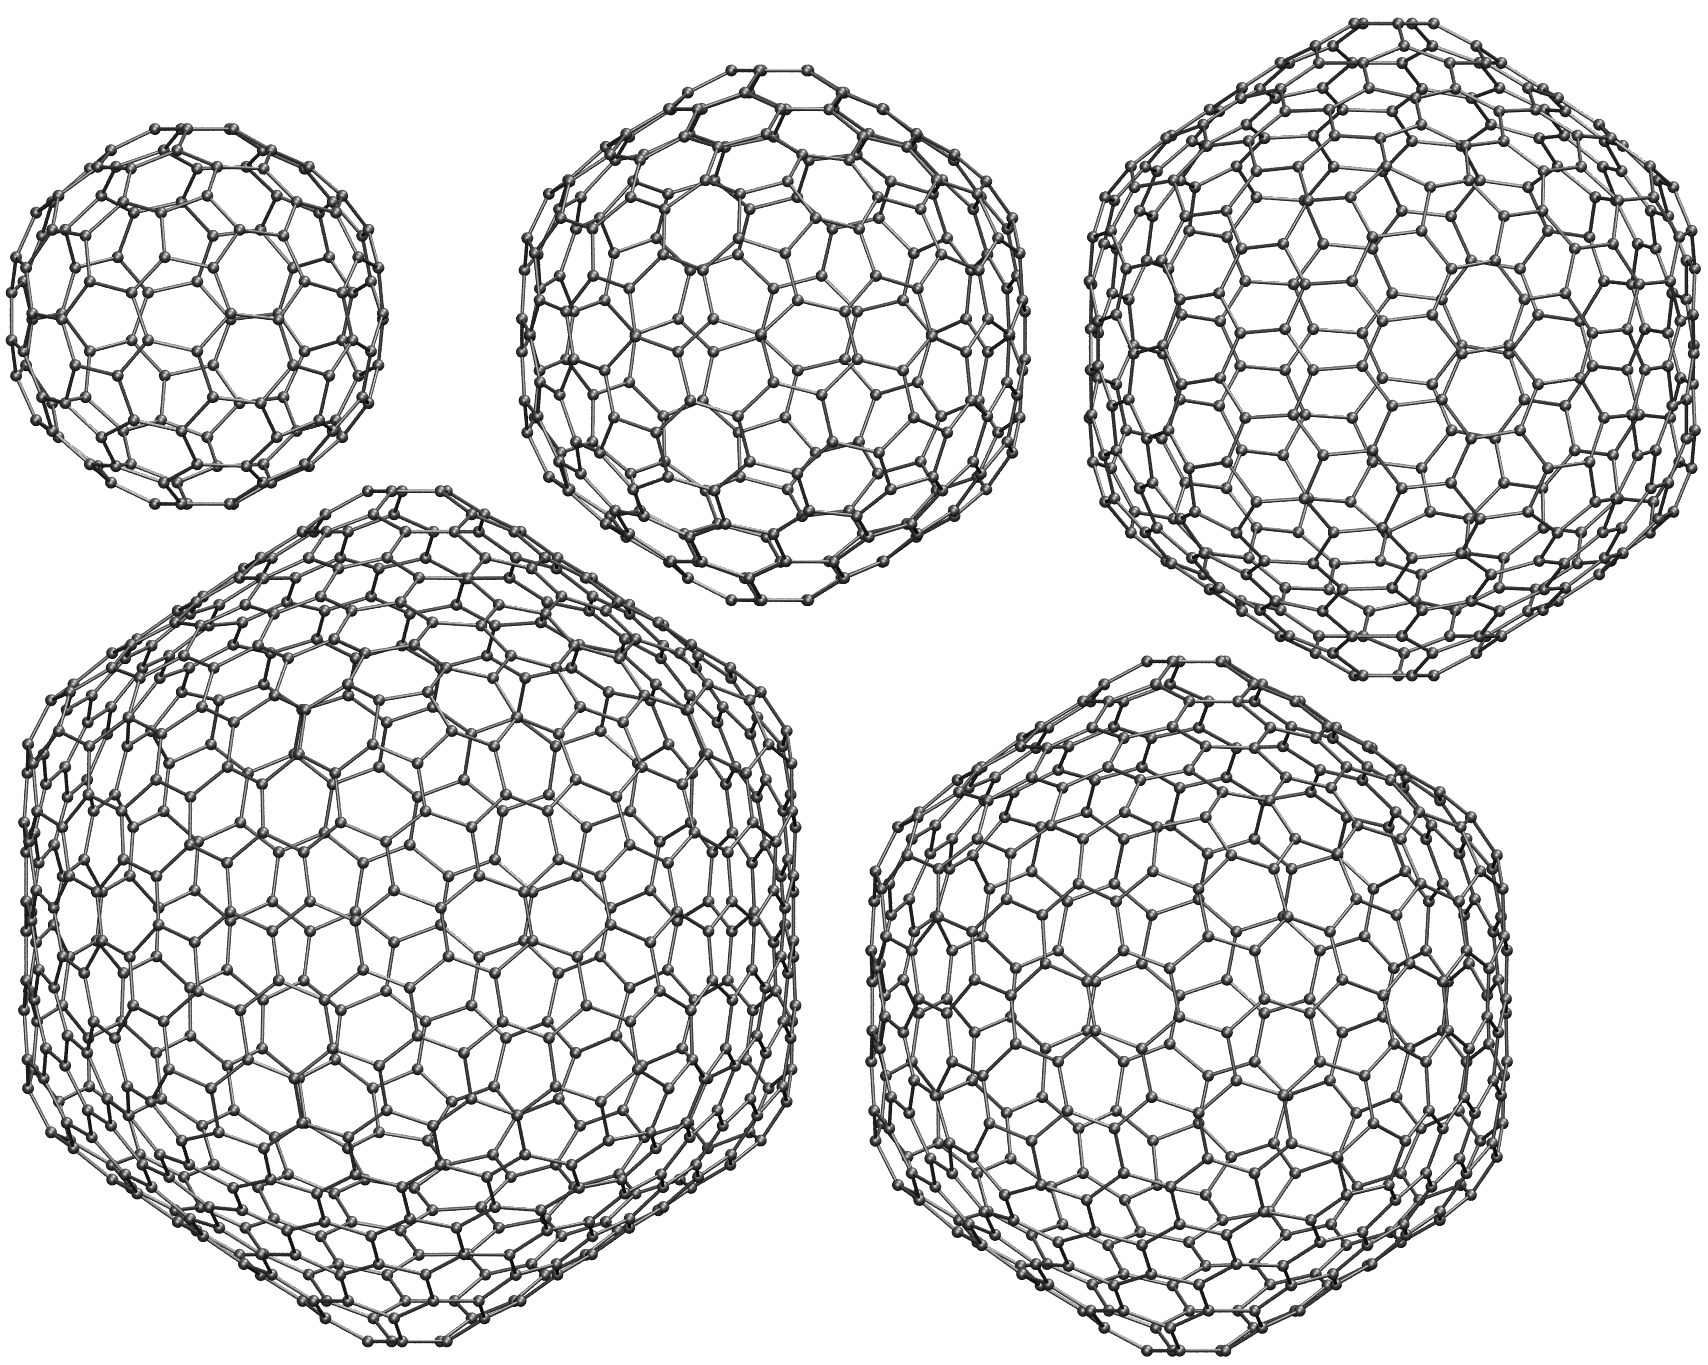
\includegraphics[width=0.6\textwidth]{carboncluster}
	\captionsetup{figurewithin = chapter}
	\captionsetup{font=small, labelfont=bf}\caption[Abbildung von ikosaedrischen Kohlenstoffclustern]{Abbildung von ikosaedrischen Kohlenstoffclustern mit \textit{I}- aber nicht \textit{I}$_\textrm{h}$-Symmetrie: C$^{2+}_{140}$ (a), C$^{2+}_{260}$ (b), C$^{2+}_{380}$ (c), C$_{420}$ (d) und C$^{2+}_{620}$ (e).}
\label{abb:carboncluster}
\end{figure}
	
\section{meta-GGA Funktionale}
In Zusammenarbeit mit Fabian Mack wurde das \texttt{mpshift} Modul um die Möglichkeit erweitert, \ac{mgga}-Funktionale bei der Berechnung von chemischen Abschirmungskonstanten zu verwenden. Die eigentliche Implementierung erfolgte dabei im Wesentlichen durch Fabian Mack. Zunächst wurden dafür die niedrig skalierenden \ac{dft} Routinen in das Modul \texttt{mpshift} übertragen und für die Berechnung von chemischen Abschirmungskonstanten angepasst. Eine kurze Beschreibung dieser niedrig skalierenden Routinen ist in Referenz \cite{deglmann2002efficient} zu finden. Die zusätzlichen Terme die bei der Funktionalableitung nach den Komponenten des Magnetfeldes bei der Verwendung von \ac{mgga}-Funktionalen (siehe Gleichung (\ref{eq:ymunudb}) bzw. (\ref{eq:mggadb})) auftreten, mussten neu programmiert werden. Dafür wurde die neue Routine \texttt{csmoper} angelegt. Im Detail ist die Implementierung sowie der Aufbau der Routine in Referenz \cite{mack2017} beschrieben. Die Genauigkeit der Berechnung von chemischen Verschiebungen mit \ac{mgga}-Funktionalen wurde für $^{13}$C, $^{19}F$ und $^{31}$P Verschiebungen getestet und mit \ac{gga} Funktionalen verglichen.\supercite{reiter2017calculation} 
	
	